\chapter{Results}  %Title of the First Chapter                                                                                 

\ifpdf
    \graphicspath{{Chapter1/Figs/Raster/}{Chapter1/Figs/PDF/}{Chapter1/Figs/}}
\else
    \graphicspath{{Chapter1/Figs/Vector/}{Chapter1/Figs/}}
\fi

%\section{Results}
%\label{sec:result}

\section{Luminosity measurement results using the pixel cluster counting method}
\section{Comparison of the luminosity results for different module veto list}
\section{Comparison of the results with other luminosity measurement techniques}
\section{Final uncertainties in PCC luminosity measurement}



\begin{figure}[!htp]
\centering
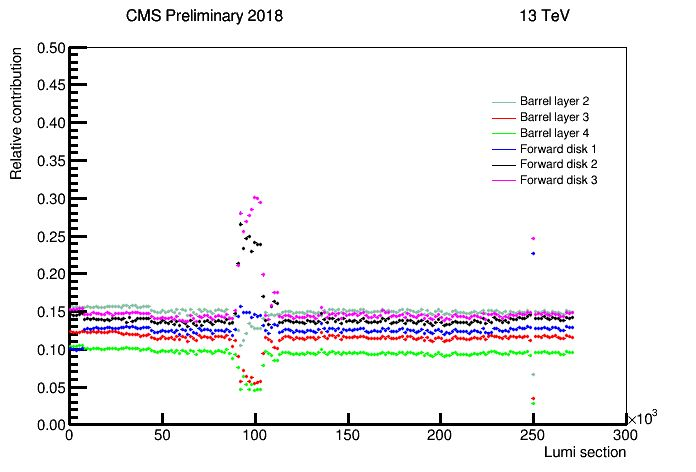
\includegraphics[width=0.8\textwidth]{ashish_thesis/pixel_layer_disk_noveto_noselection.png}
\caption{%                                                                                                                                                                                                            
   Luminosity fraction of pixel detector for various layer and disks as a function of lumi section after removing low statistics lumi section.
}
\label{fig:PCC_stab_begin}
\end{figure}





\begin{figure}[!htp]
\centering
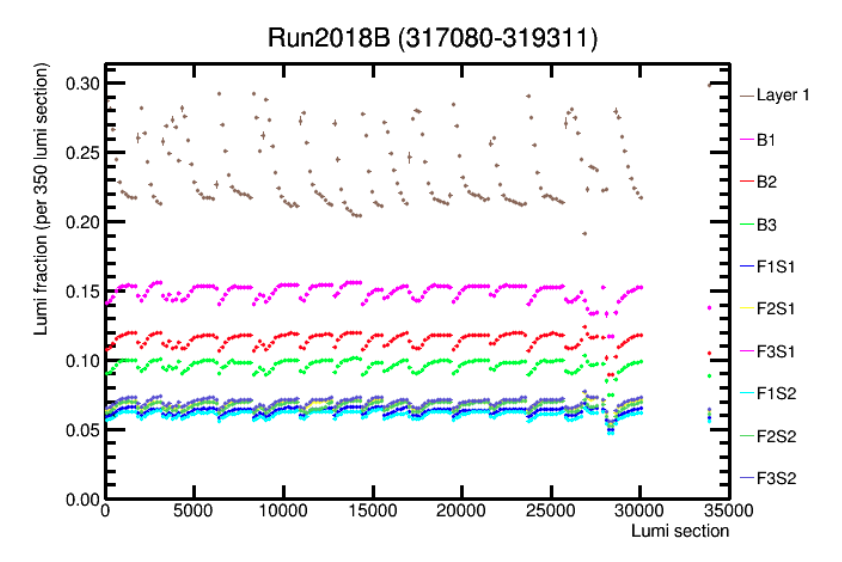
\includegraphics[width=0.8\textwidth]{ashish_thesis/pcc_stability_begin.png}
\caption{%
   Luminosity fraction of pixel detector for various layer and disks as a function of lumi section after removing low statistics lumi section.
}
\label{fig:PCC_stab_begin}
\end{figure}




\begin{figure}[!htp]
\centering
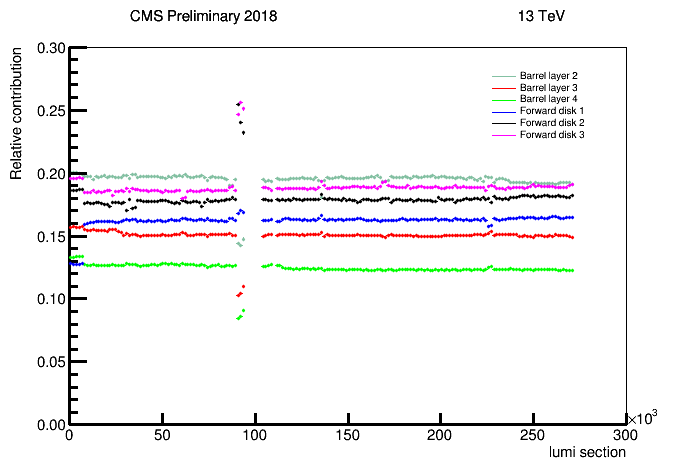
\includegraphics[width=0.8\textwidth]{ashish_thesis/pcc_frac_L0_veto.png}
\caption{%                                                                                                                                                                                                            
   Luminosity fraction of pixel detector for various layer and disks as a function of lumi section after removing low statistics lumi section.
}
\label{fig:PCC_stab_L0_veto}
\end{figure}




\begin{figure}[!htp]
\centering
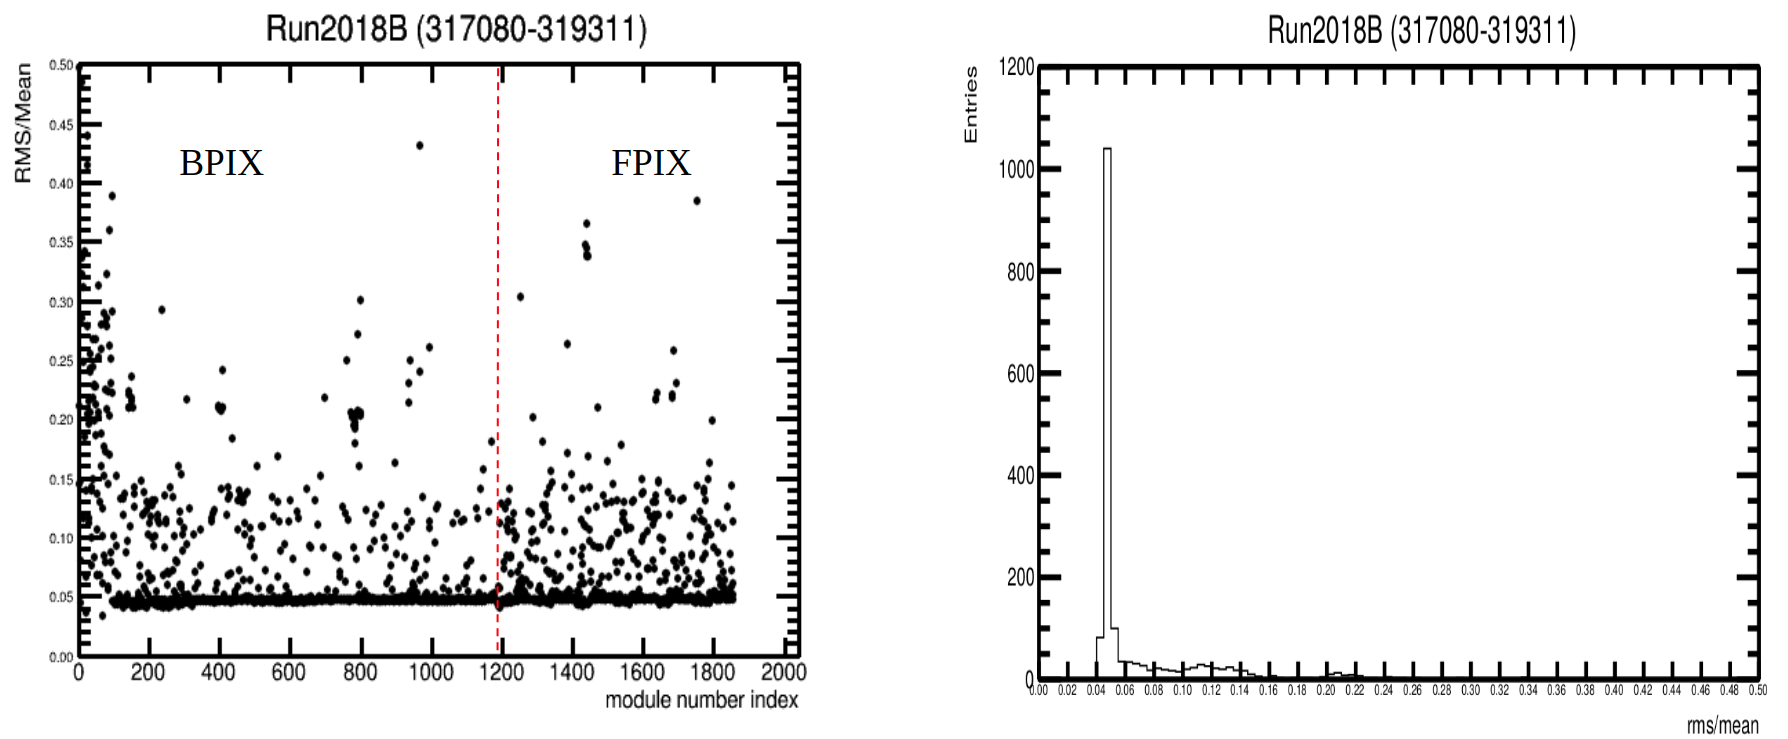
\includegraphics[width=1\textwidth]{ashish_thesis/rms_mean_all_modules_B.png}
\caption{%
   Mean and rms values are obtained from module weight distribution by obtaining its y projection to plot rms/mean as a function of module number index.
}
\label{fig:rms_mean_B}
\end{figure}




\begin{figure}[!htp]
\centering
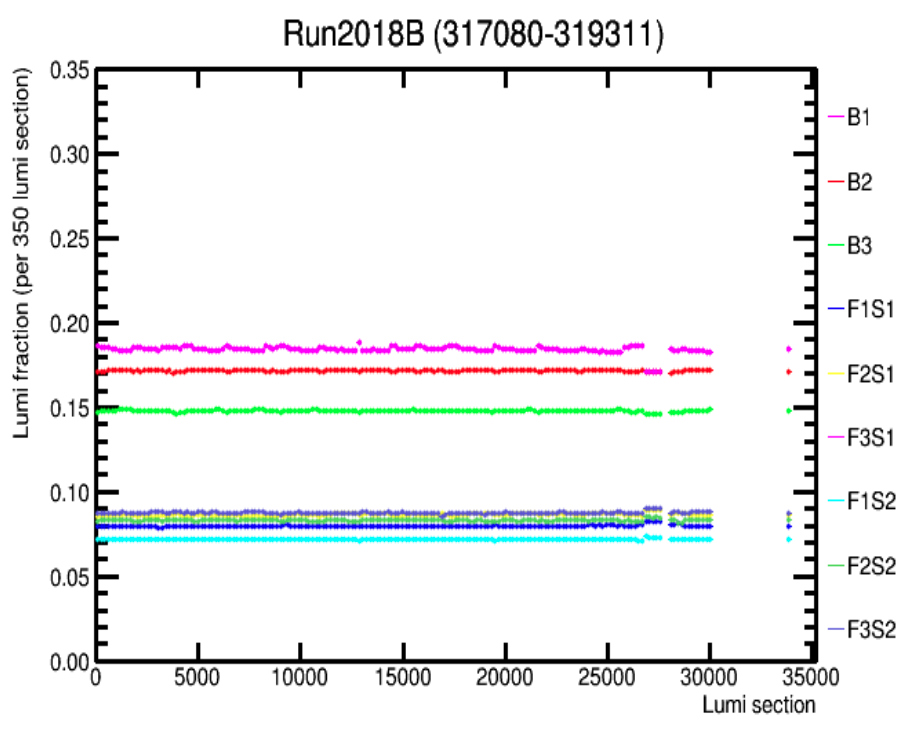
\includegraphics[width=0.7\textwidth]{ashish_thesis/first_iteration_stability.png}
\caption{%
   Luminosity fractions of various layer and disk after applying 7\% loose selection.
}
\label{fig:f_it_stability}
\end{figure}

\begin{figure}[!htp]
\centering
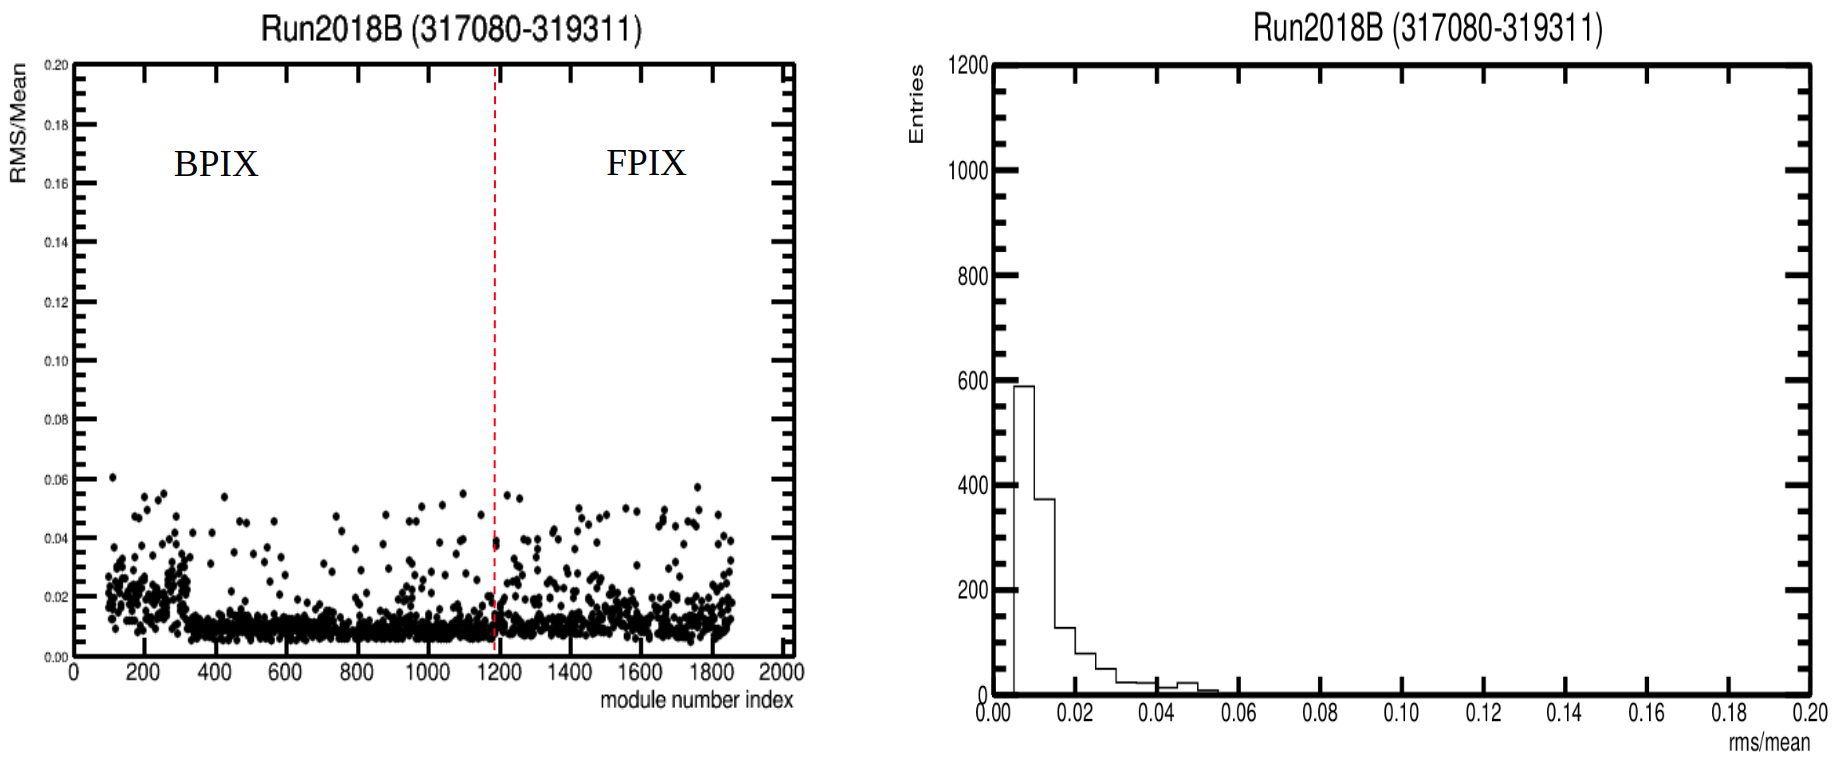
\includegraphics[width=1\textwidth]{ashish_thesis/remaining_second_iteration.png}
\caption{%
 rms/mean of module stability profile after applying 7\% loose cut.
}
\label{fig:sec_it_remain}
\end{figure}


\begin{figure}[!htp]
\centering
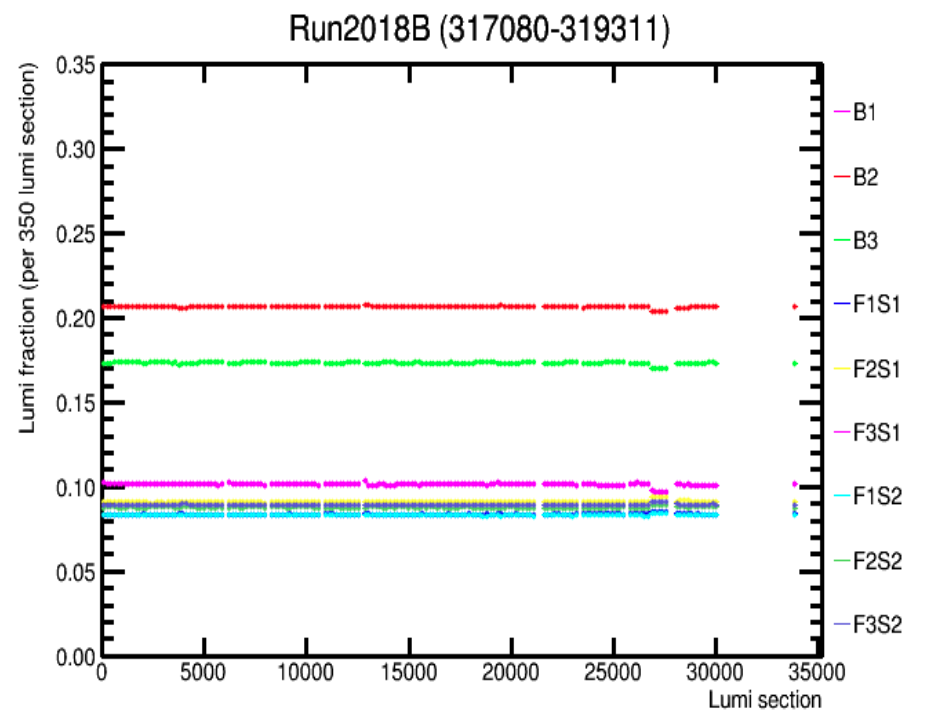
\includegraphics[width=0.7\textwidth]{ashish_thesis/second_iteration_stability.png}
\caption{%
   Luminosity fraction after applying third selection of 2\% on rms/mean values to removed tail. After final iteration, profile for layers and disks is very stable. Only one Fill around lumi section 27000 shows instability.
}
\label{fig:sec_it_stability}
\end{figure}

\begin{figure}[!htp]
\centering
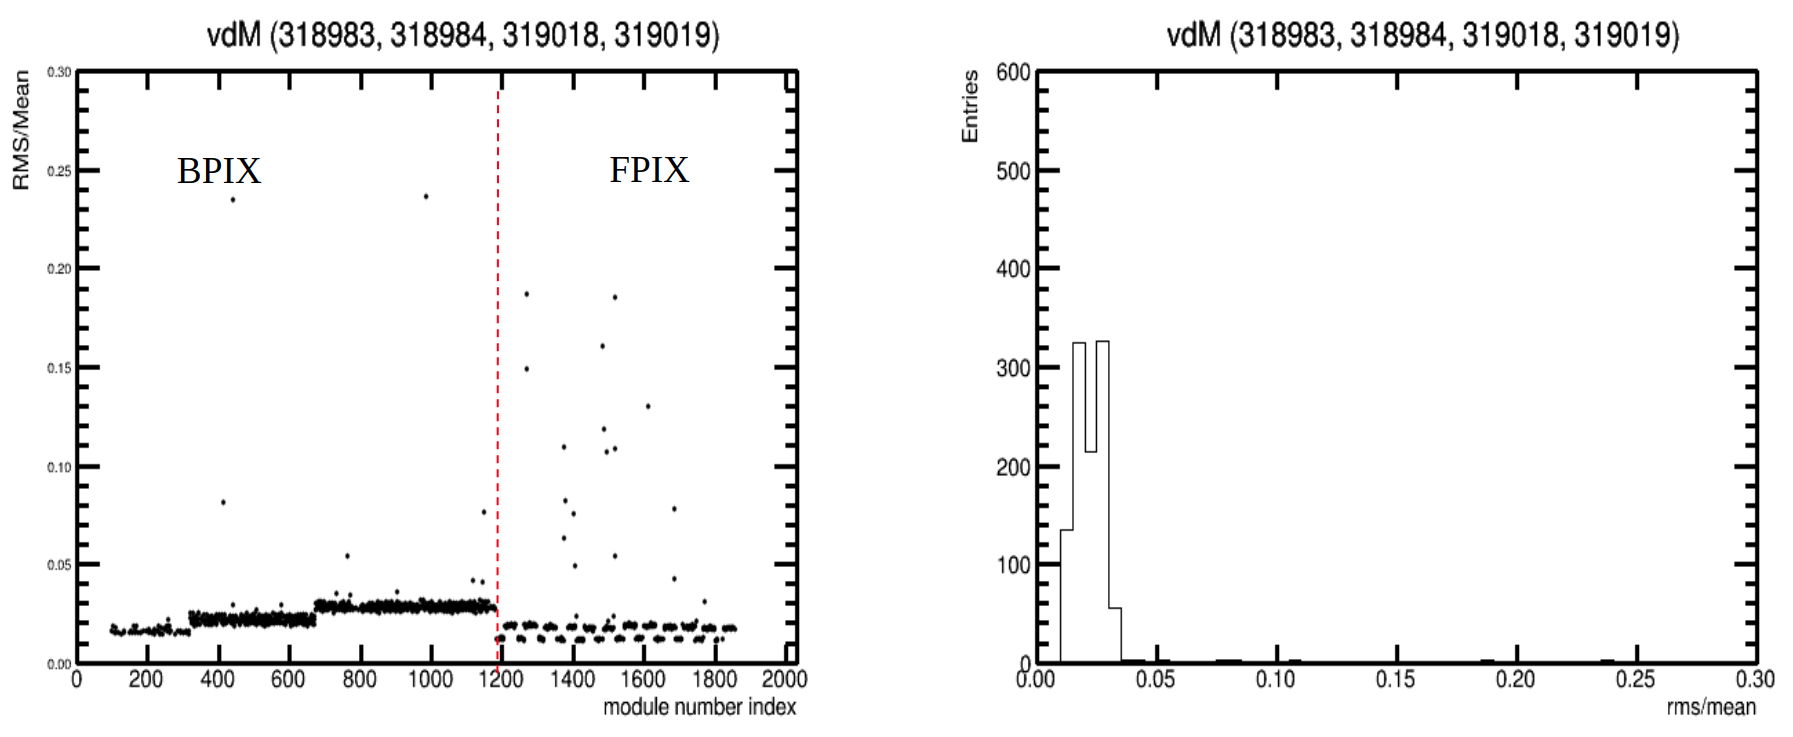
\includegraphics[width=1\textwidth]{ashish_thesis/vdm_rms_mean.png}
\caption{%
   rms/mean values of module stability profile for vdM data. 
}
\label{fig:vdm_cut}
\end{figure}


\begin{figure}[!htp]
\centering
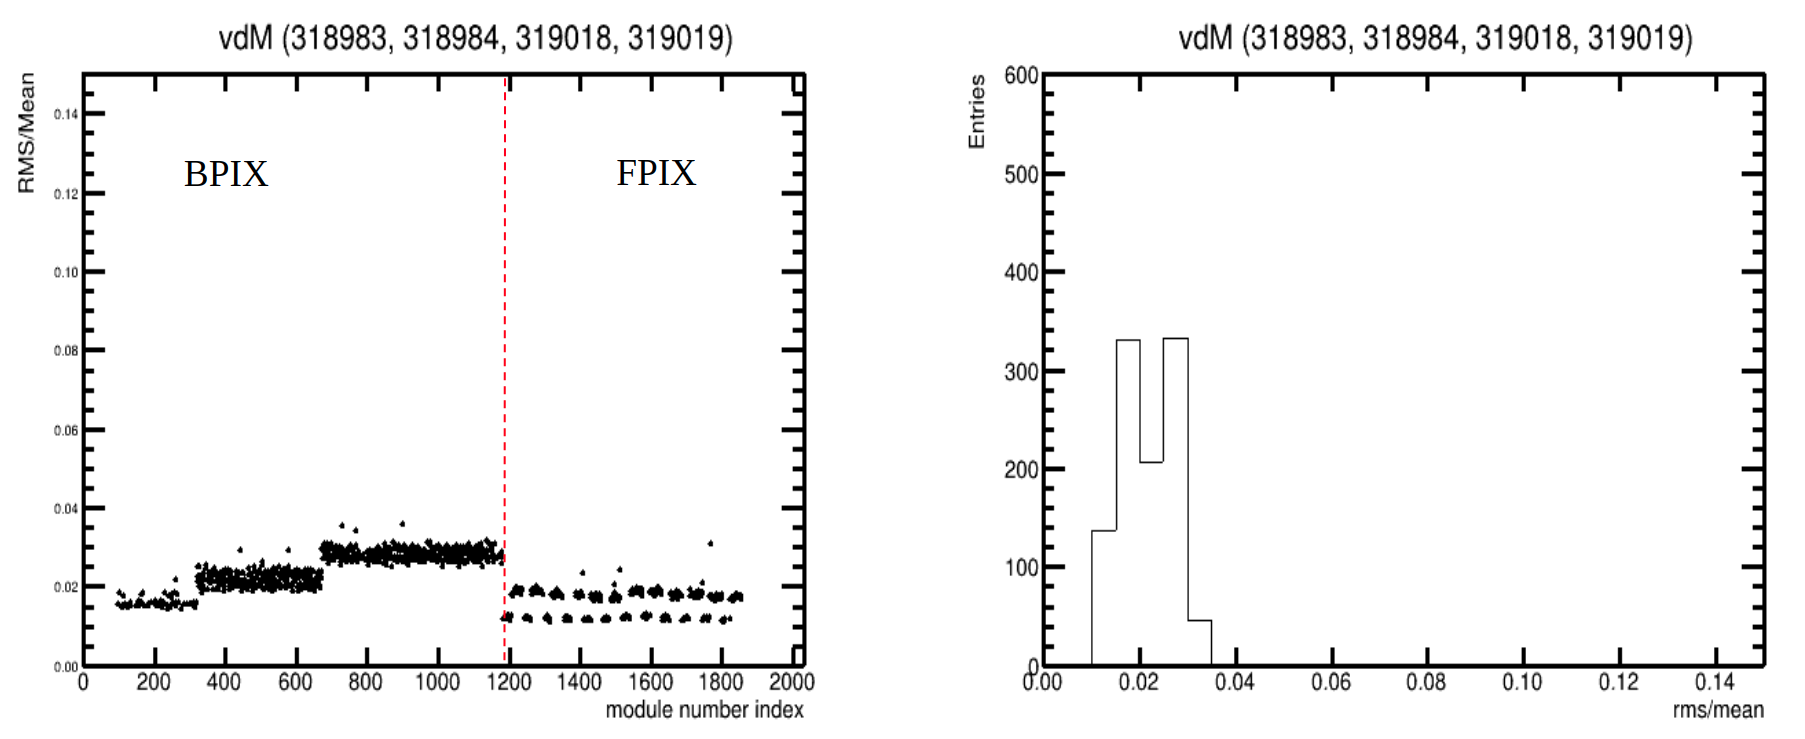
\includegraphics[width=1\textwidth]{ashish_thesis/first_iteration_vdm.png}
\caption{%
   rms/mean values of module stability profile after applying a selection of 4\% cut . 
}
\label{fig:vdm_cut}
\end{figure}


\begin{figure}[!htp]
\centering
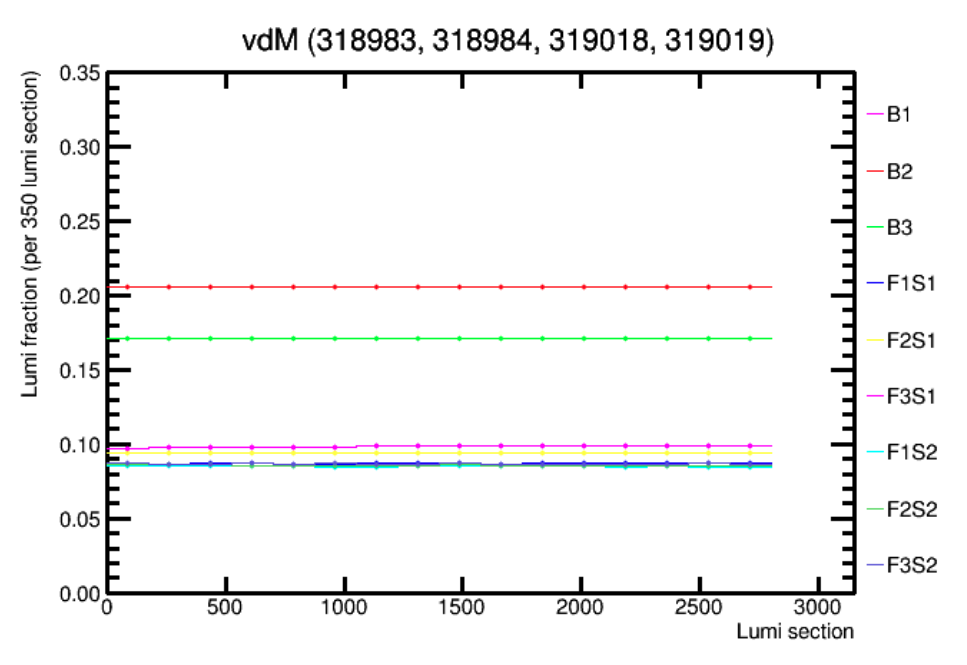
\includegraphics[width=0.7\textwidth]{ashish_thesis/vdm_stability.png}
\caption{%
   Pixel layer and disk for vdM data shows excellent stability with the 2\% rms module veto list consisting of 800 bad modules. After applying module veto list from physics run period B on top of module veto list formed by outliers, pixel layers and disks luminosity ratios shows excellent stability.
}
\label{fig:vdm_stability}
\end{figure}


\begin{figure}[!htp]
\centering
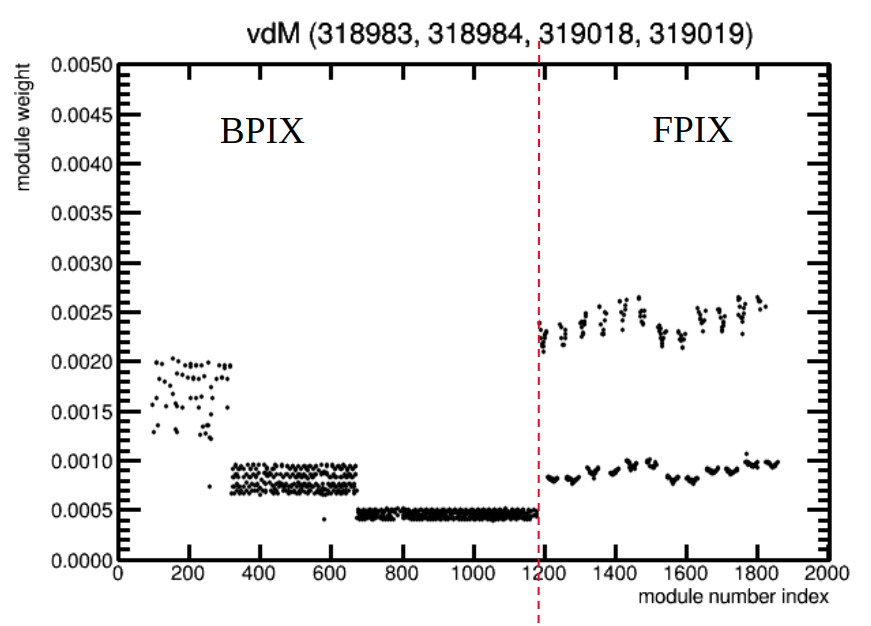
\includegraphics[width=0.7\textwidth]{ashish_thesis/module_weights_per_period_veto.png}
\caption{%
   Module weights for 2\% rms module vetolist consisting of 800 good modules and 1056 bad modules.
}
\label{fig:mod_weight_new_veto}
\end{figure}


\begin{figure}[!htp]
\centering
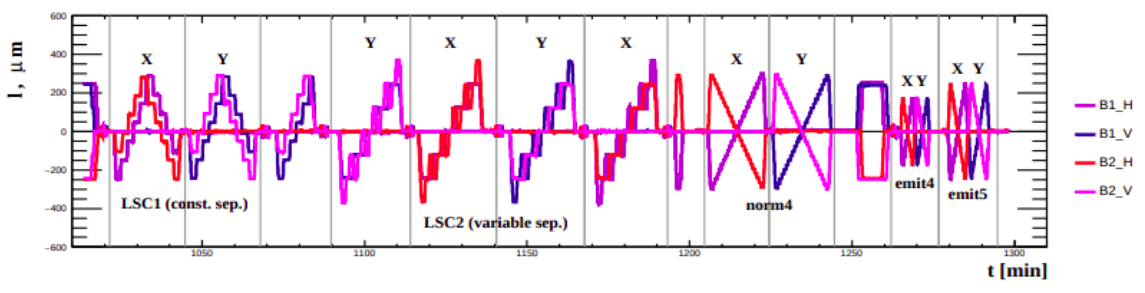
\includegraphics[width=0.8\textwidth]{ashish_thesis/vdm_beam_position.png}
\caption{%
   X and Y positions of two beams showing length scale scans, vdM scans and emittance scans.
}
\label{fig:beam_plot_vdm}
\end{figure}


\begin{figure}[!htp]
\centering
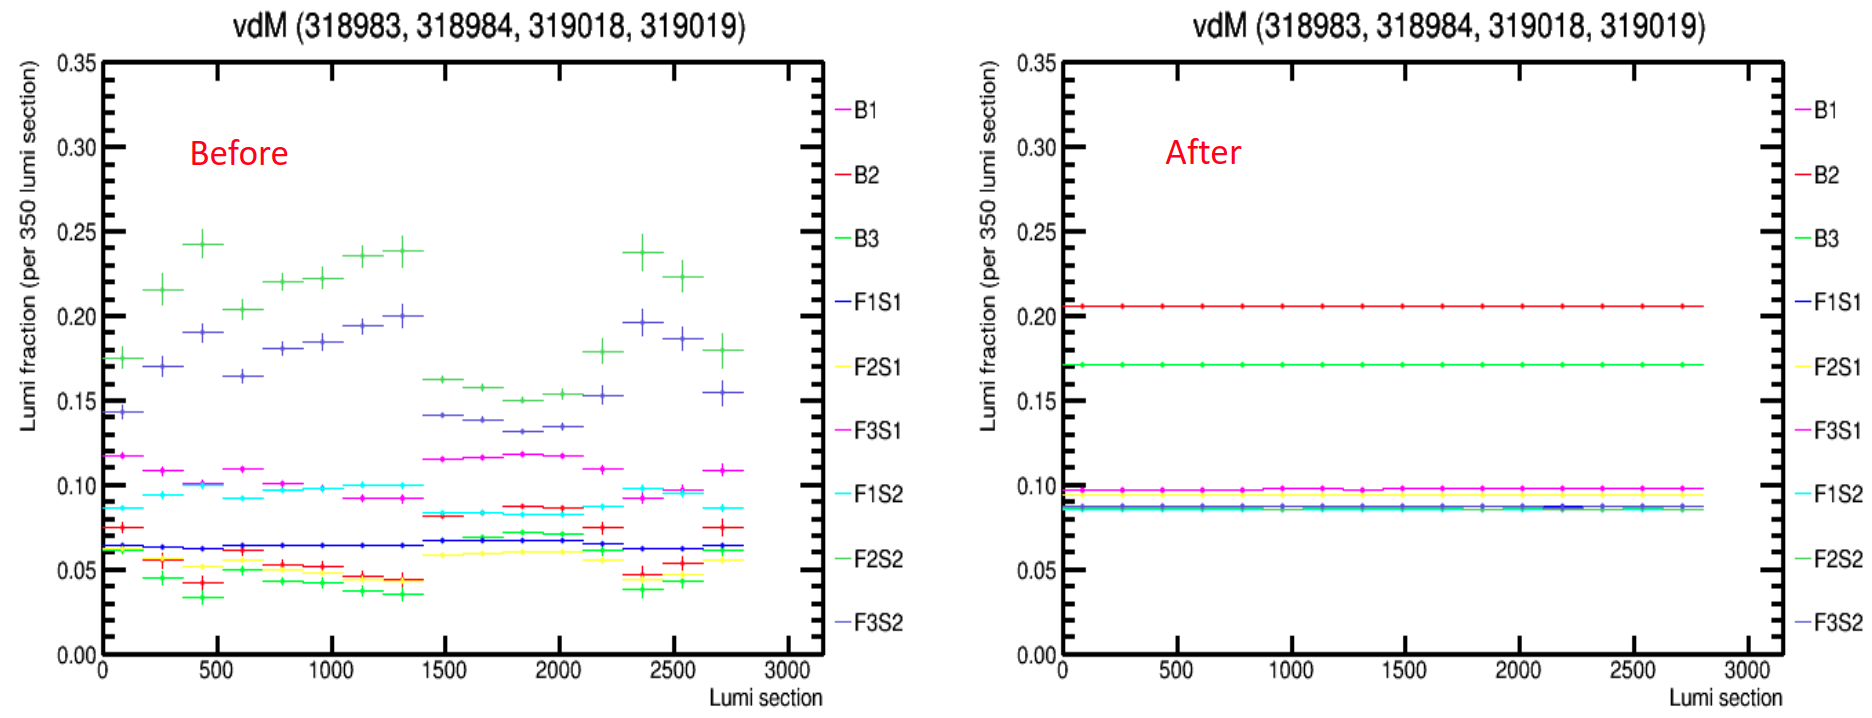
\includegraphics[width=1\textwidth]{ashish_thesis/before_after_vdm_stability.png}
\caption{%
   Luminosity fraction (stability plots) before and after applying 2\% rms module vetolist.
}
\label{fig:b_a_stability_vdm}
\end{figure}


\begin{figure}[!htp]
\centering
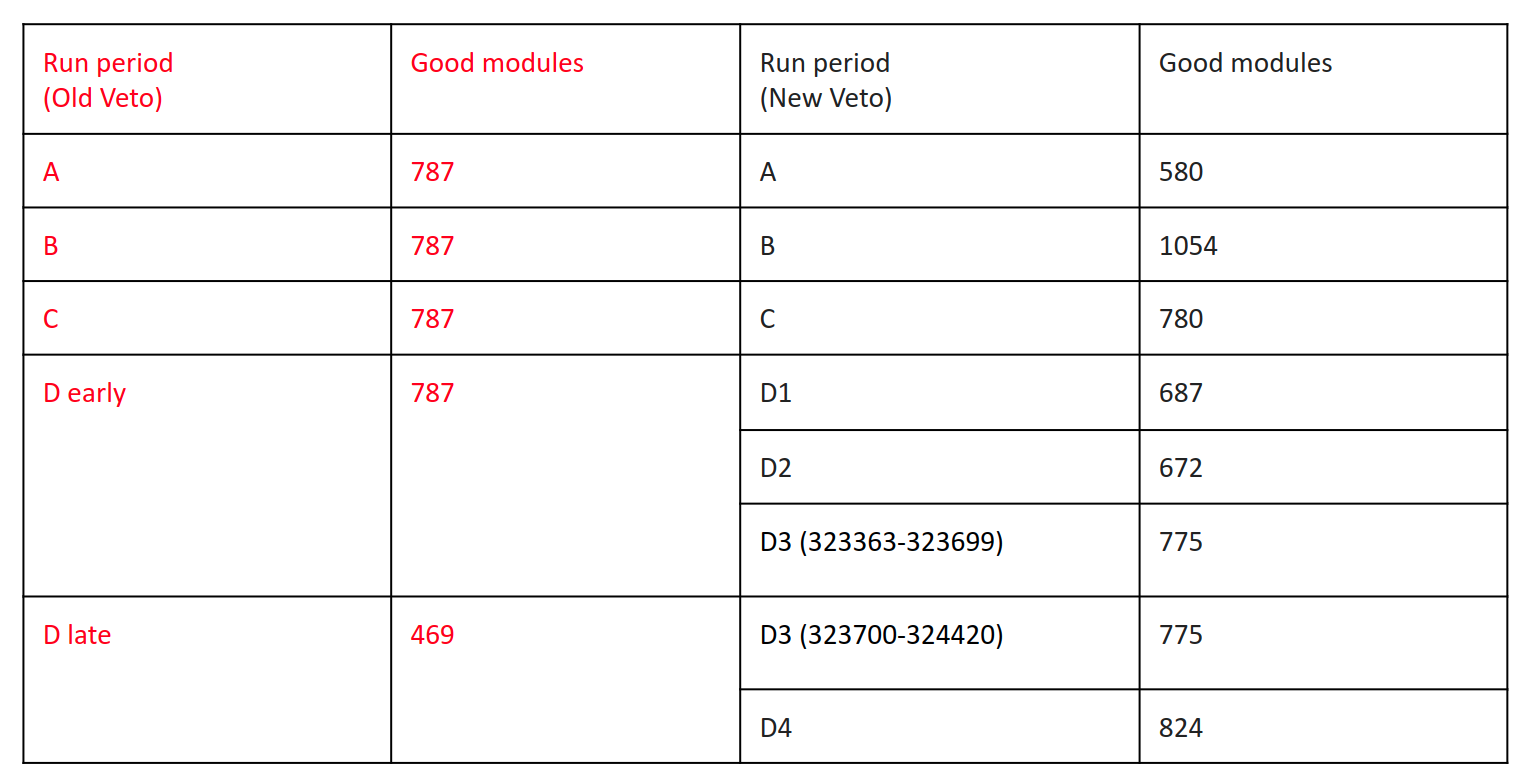
\includegraphics[width=0.8\textwidth]{ashish_thesis/old_new_veto.png}
\caption{%
   klm
}
\label{fig:old_new_vetolist}
\end{figure}

\begin{figure}[!htp]
\centering
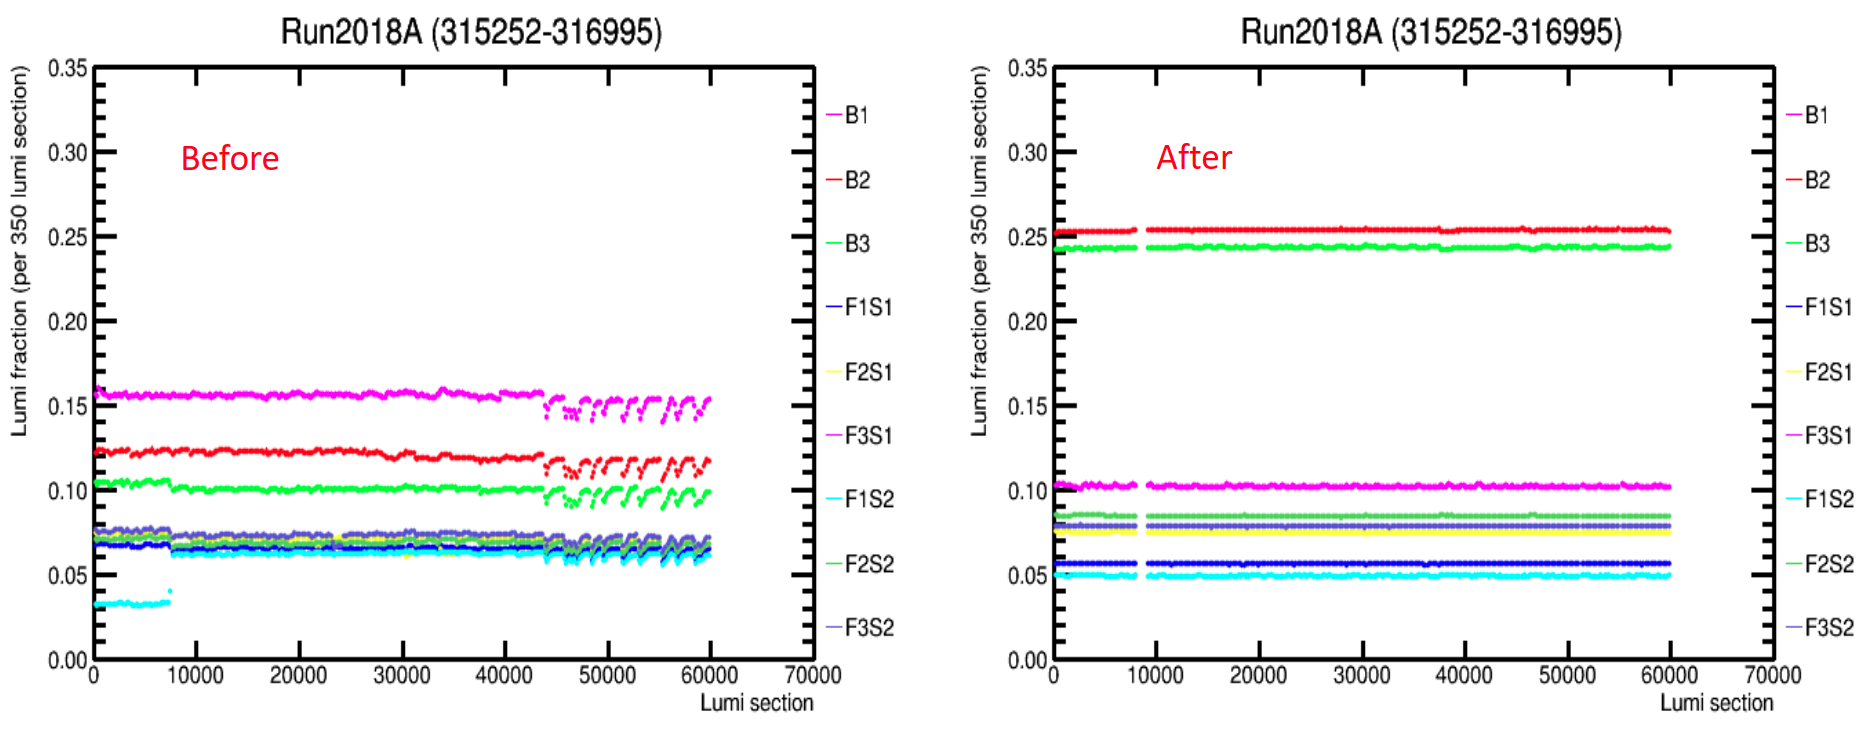
\includegraphics[width=1\textwidth]{ashish_thesis/2018A_before_after_stability.png}
\caption{%
   Stability plots for period A before and after applying module vetolist.
}
\label{fig:stability_A}
\end{figure}

\begin{figure}[!htp]
\centering
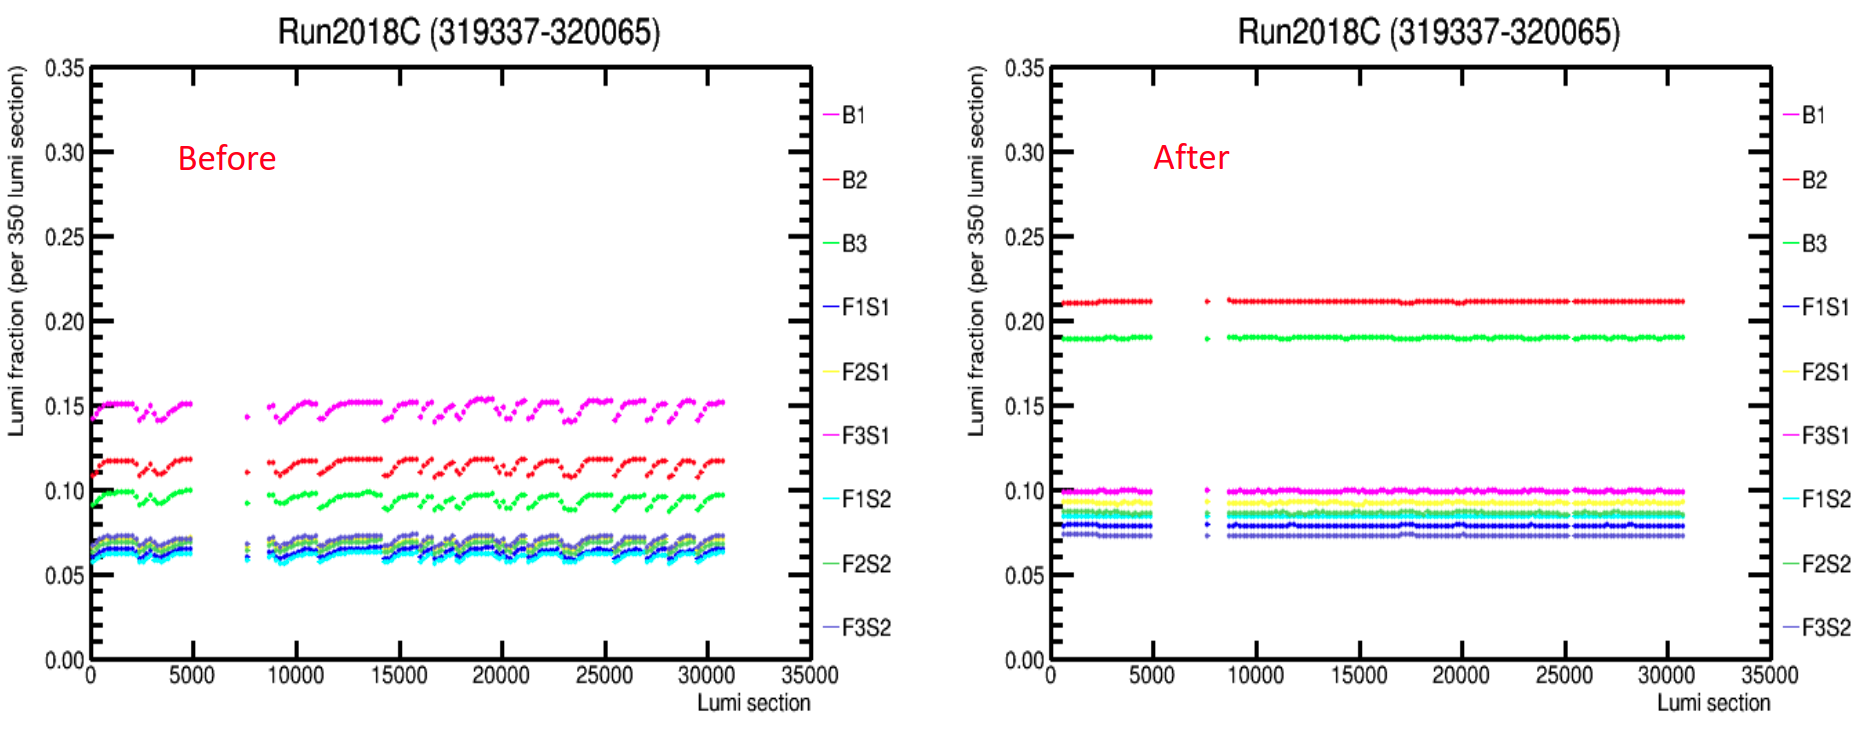
\includegraphics[width=1\textwidth]{ashish_thesis/Run2018C_before_after_stability.png}
\caption{%
  Stability plots for period C before and after applying module vetolist.
}
\label{fig:stability_C}
\end{figure}


\begin{figure}[!htp]
\centering
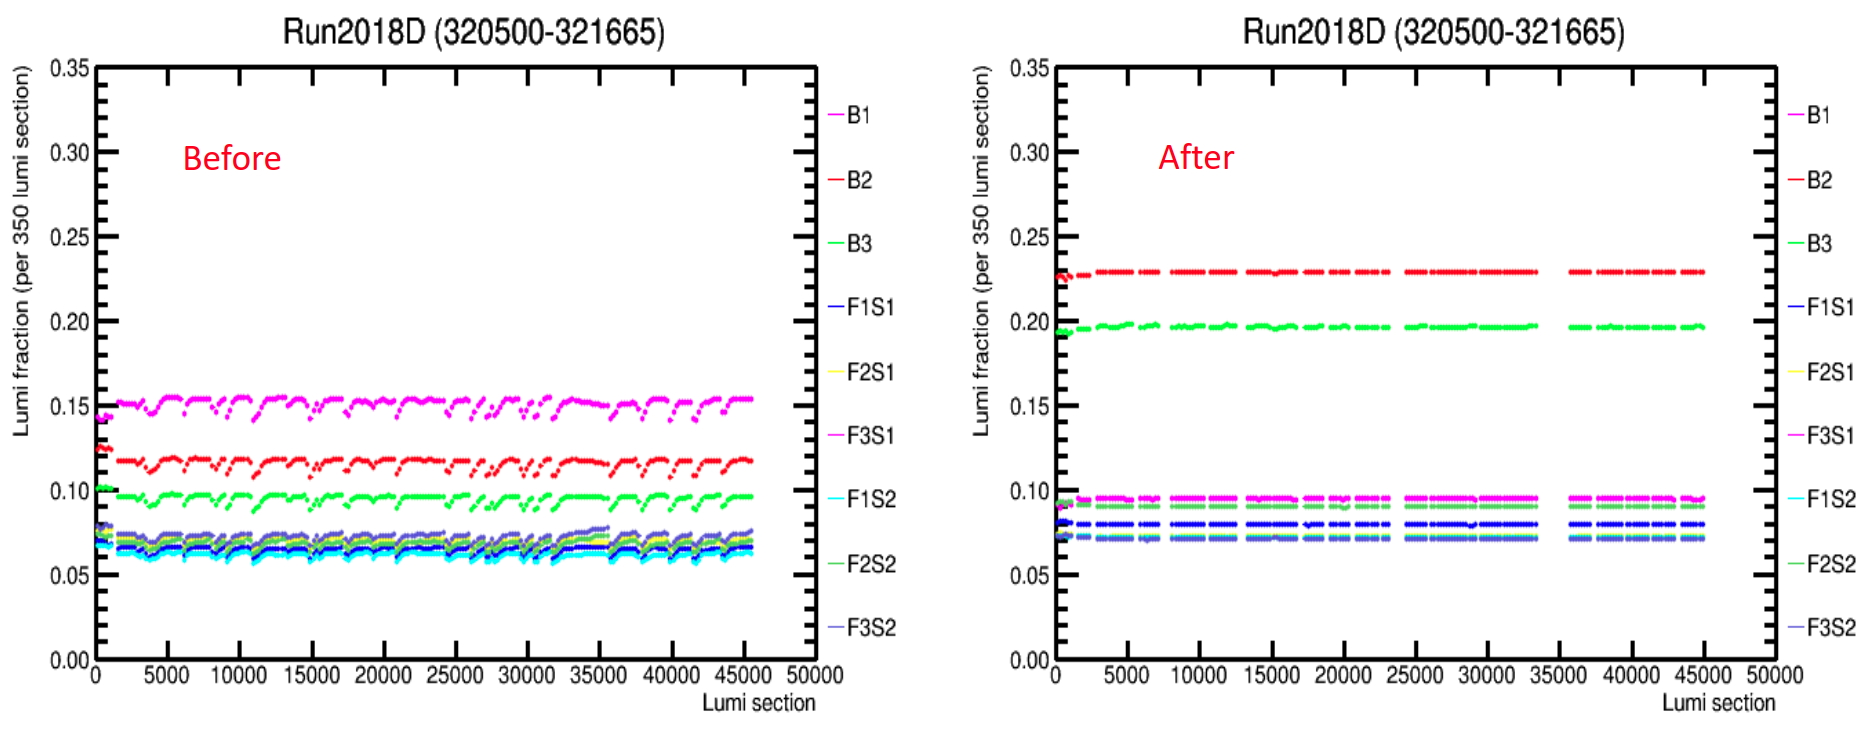
\includegraphics[width=1\textwidth]{ashish_thesis/Run2018D1_before_after_stability.png}
\caption{%
   Stability plots for period D1 before and after applying module vetolist.
}
\label{fig:stability_D1}
\end{figure}


\begin{figure}[!htp]
\centering
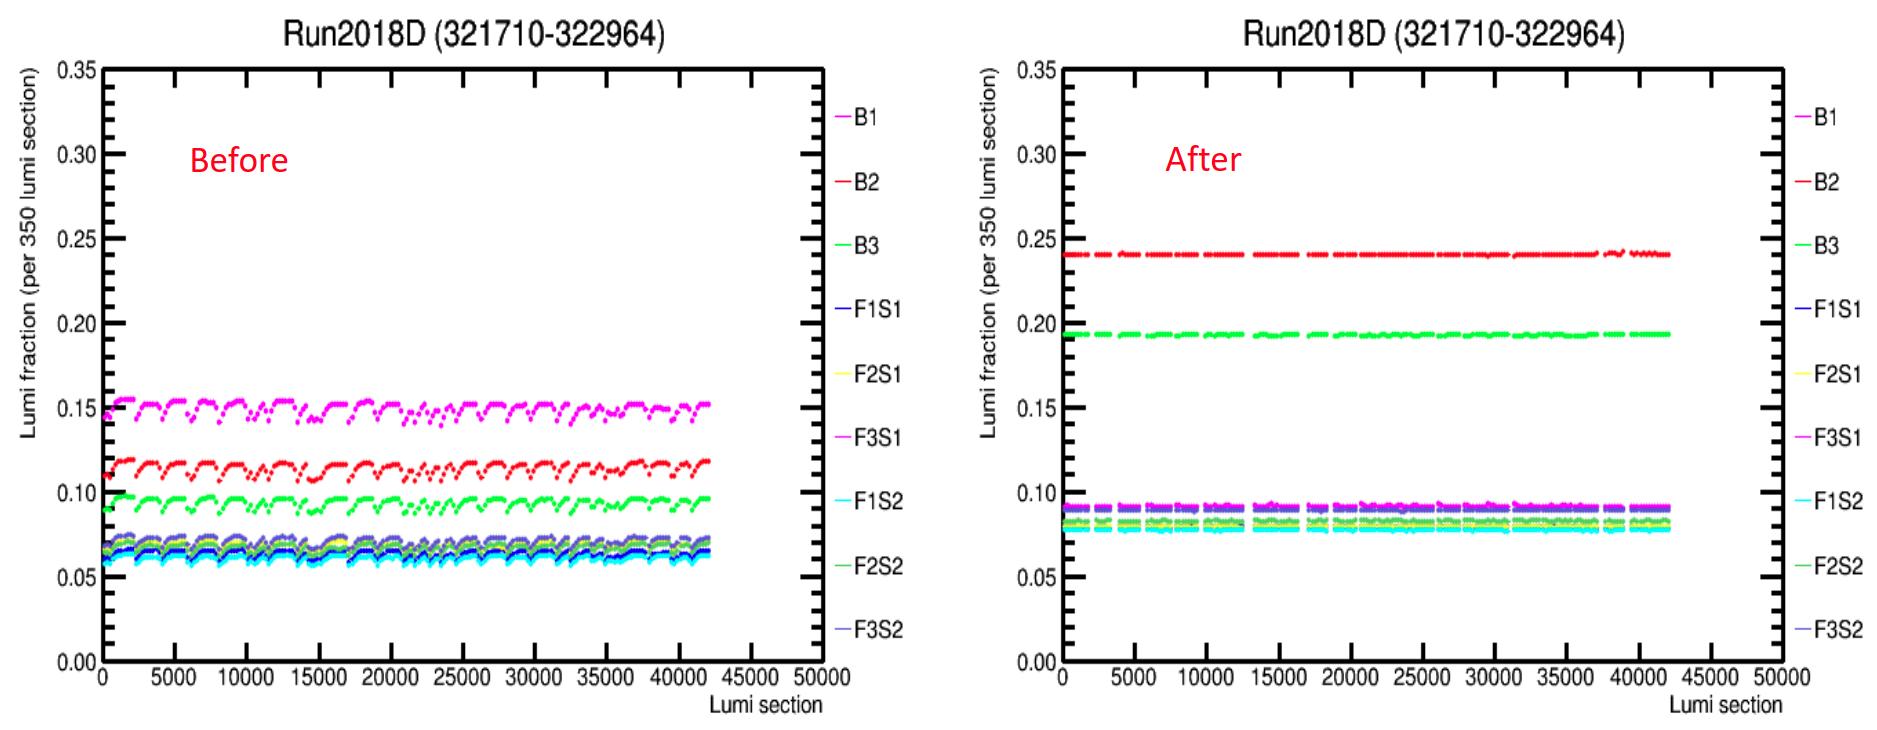
\includegraphics[width=1\textwidth]{ashish_thesis/Run2018D2_before_after_stability.png}
\caption{%
   Stability plots for period D2 before and after applying module vetolist.
}
\label{fig:stability_D2}
\end{figure}


\begin{figure}[!htp]
\centering
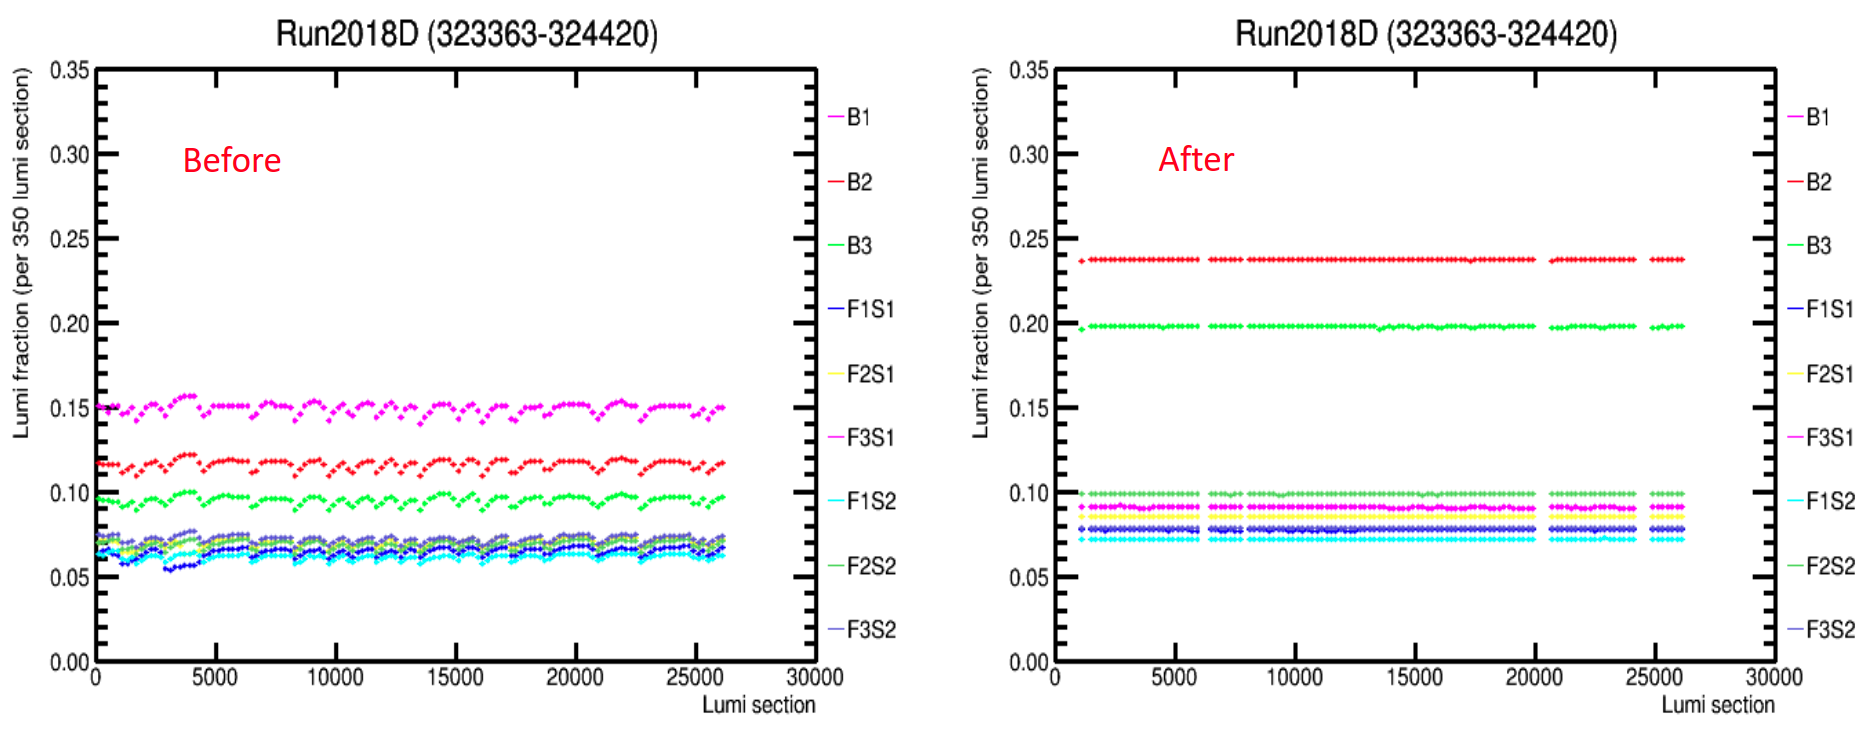
\includegraphics[width=1\textwidth]{ashish_thesis/Run2018D3_before_after_stability.png}
\caption{%
   Stability plots for period D3 before and after applying module vetolist.
}
\label{fig:stability_D3}
\end{figure}


\begin{figure}[!htp]
\centering
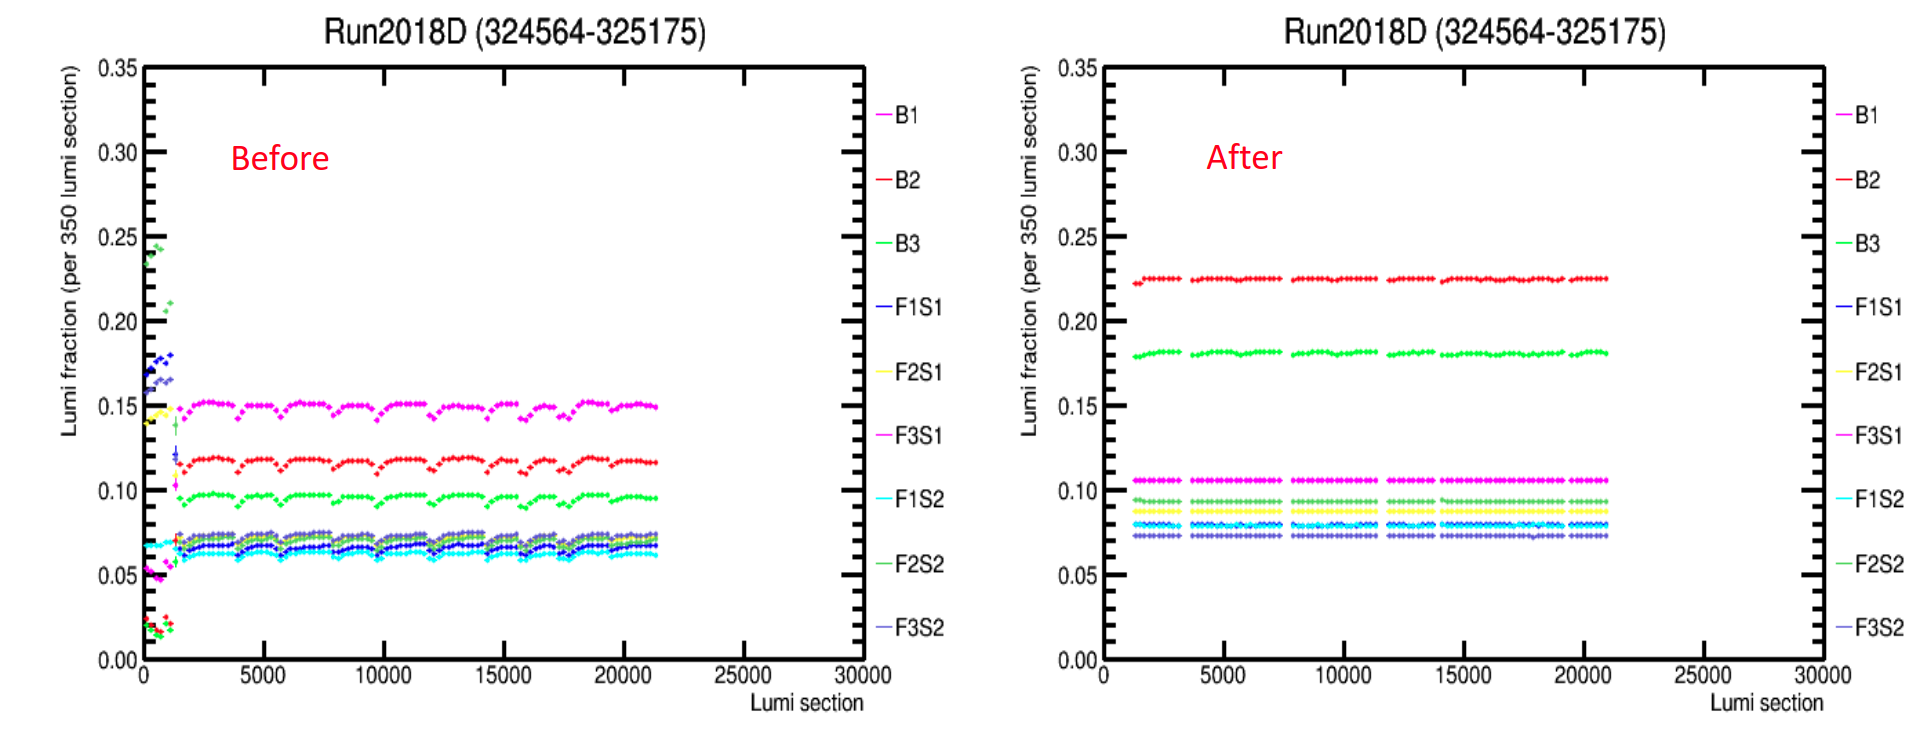
\includegraphics[width=1\textwidth]{ashish_thesis/Run2018D4_before_after_stability.png}
\caption{%
   Stability plots for period D4 before and after applying module vetolist.
}
\label{fig:stability_D4}
\end{figure}


\begin{figure}[!htp]
\centering
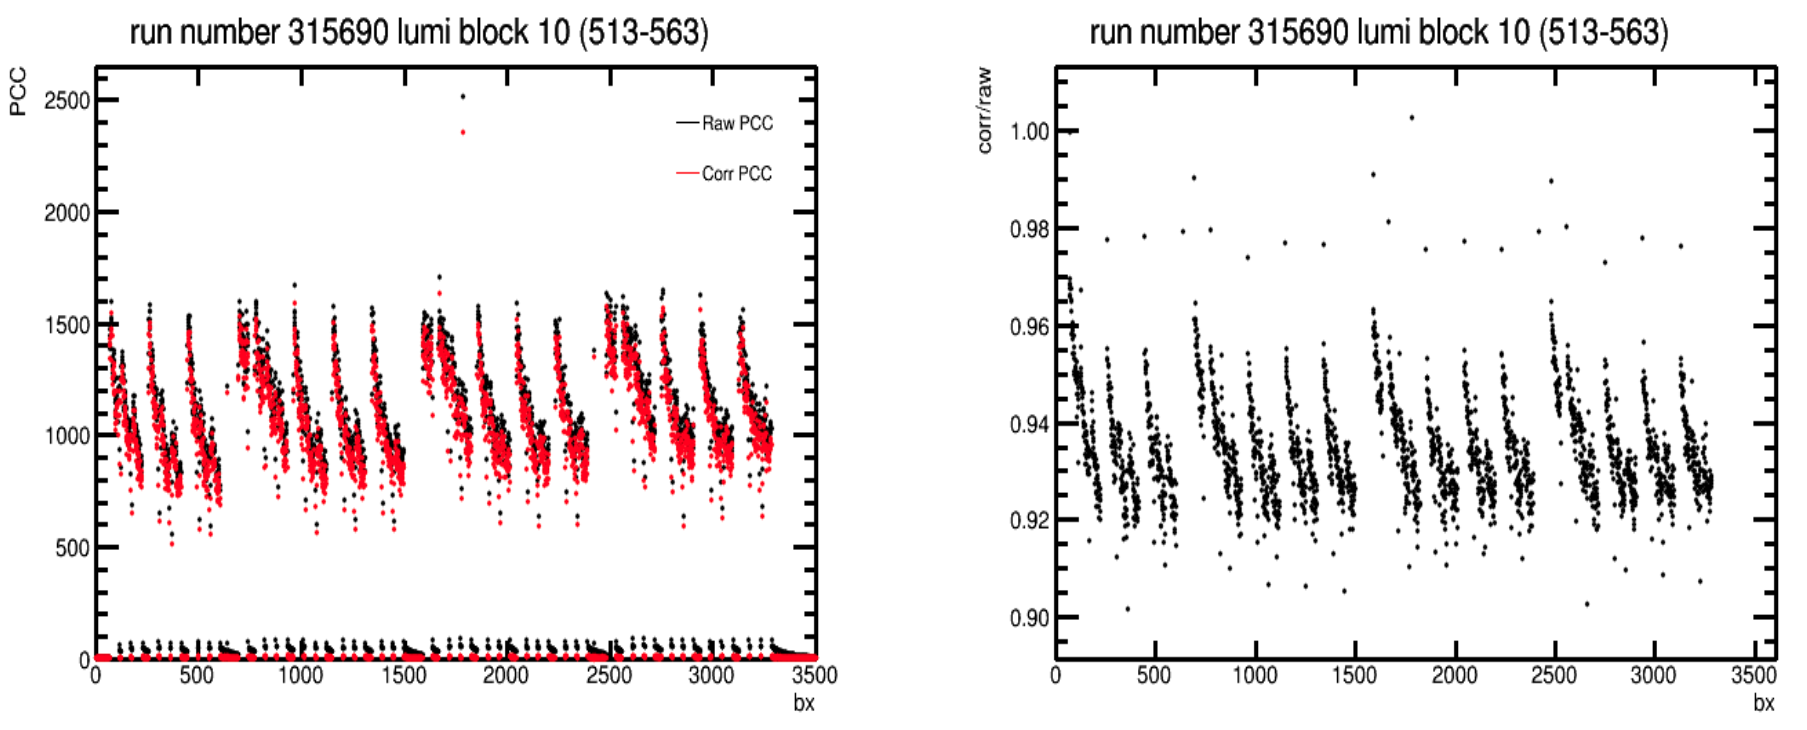
\includegraphics[width=1\textwidth]{ashish_thesis/raw_corr_hist.png}
\caption{%
   Raw and corrected PCC with its ratio.
}
\label{fig:stability_D5}
\end{figure}


\begin{figure}[!htp]
\centering
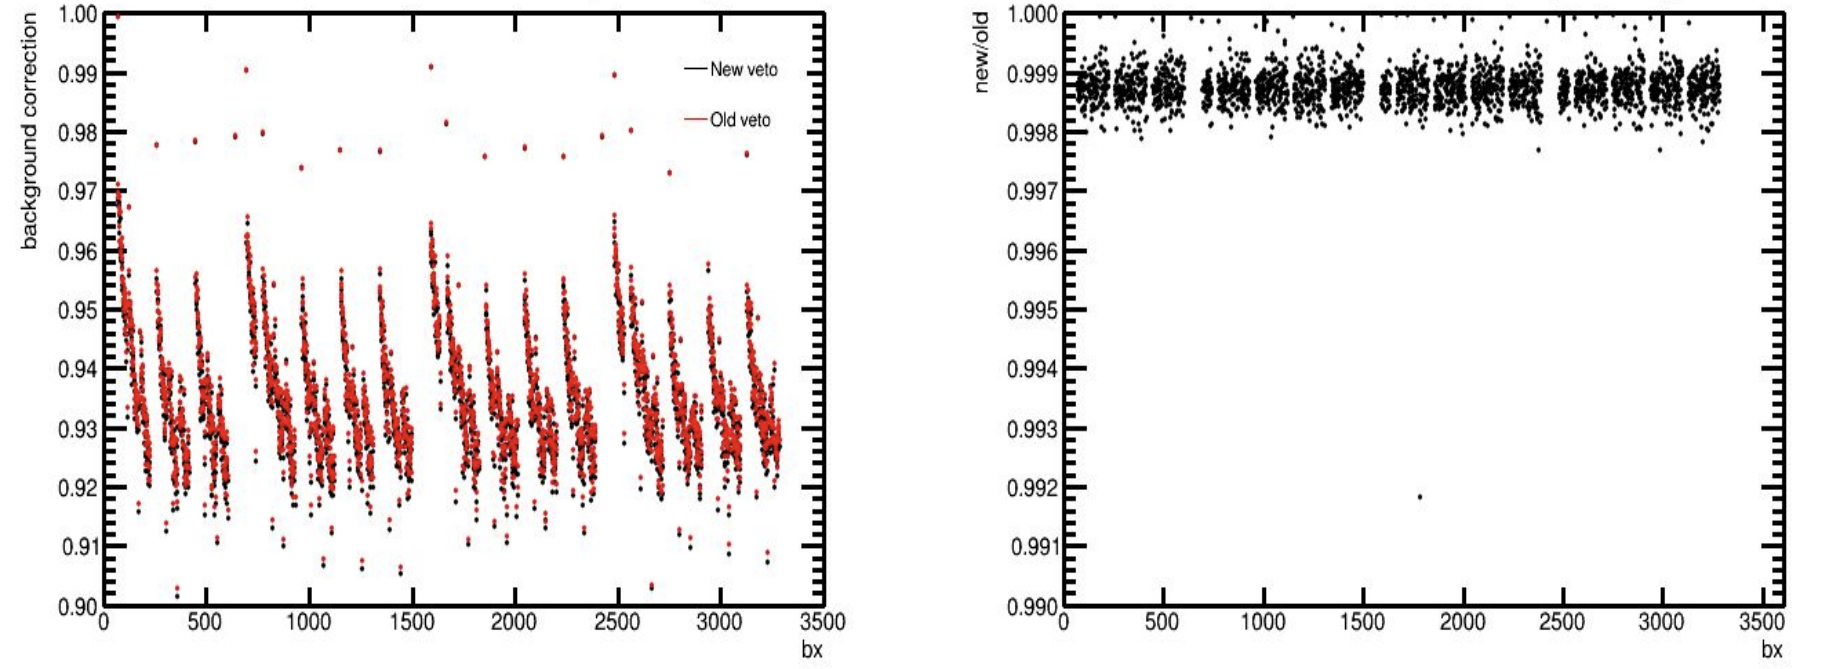
\includegraphics[width=1\textwidth]{ashish_thesis/veto_change_same_af.png}
\caption{%                                                                                                                                                                                                            
    ratio of scale factor for new and old veto.
}
\label{fig:af_change_veto}
\end{figure}



\begin{figure}[!htp]
\centering
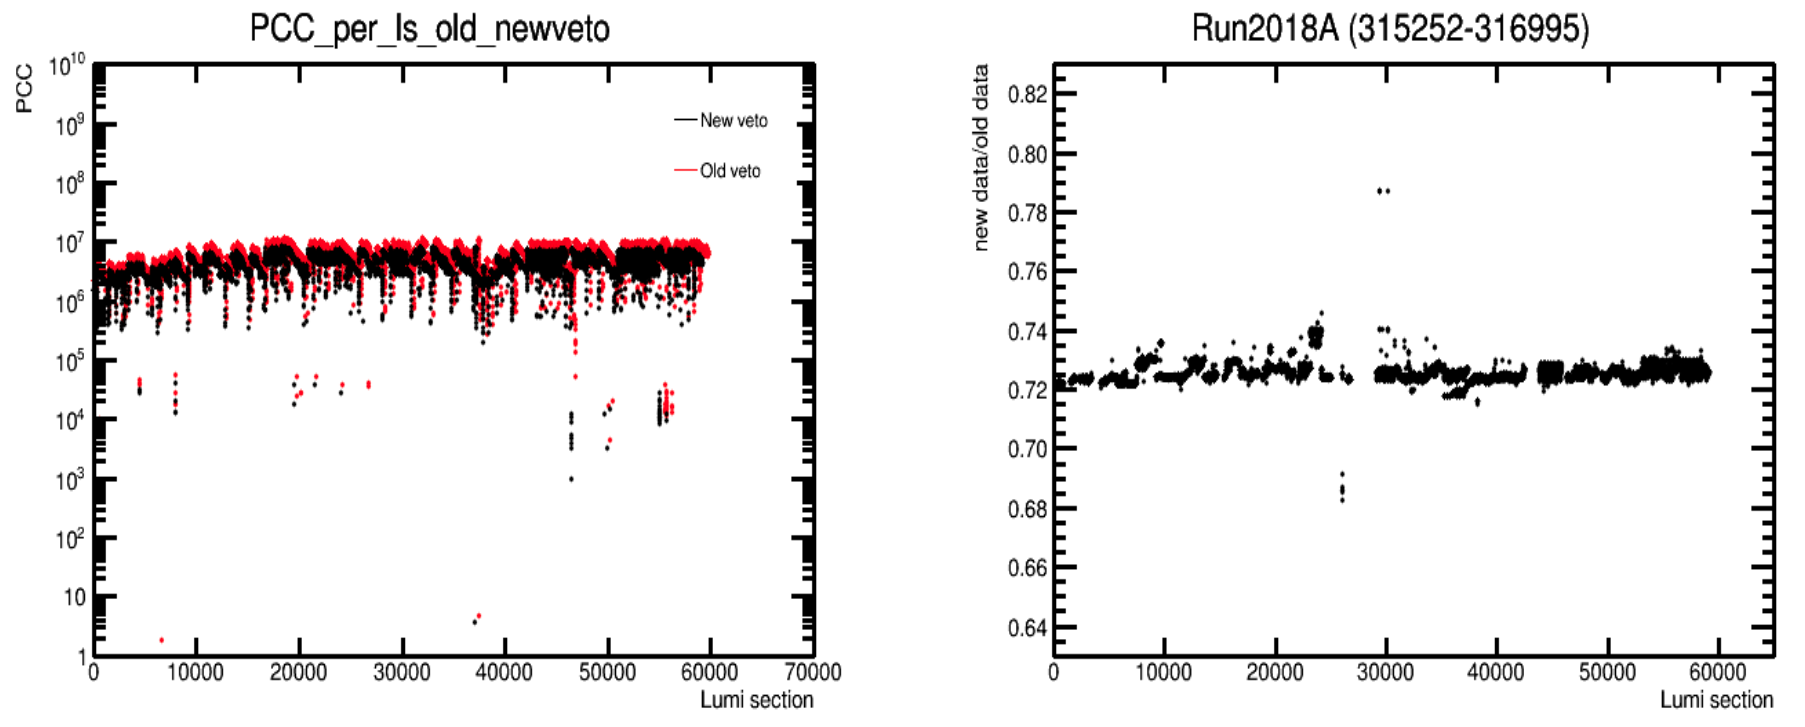
\includegraphics[width=1\textwidth]{ashish_thesis/Run2018A_old_new_veto.png}
\caption{%
   PCC as a function of lumi section for old and new vetolist with its ratio for period A.
}
\label{fig:old_new_veto_A}
\end{figure}

\begin{figure}[!htp]
\centering
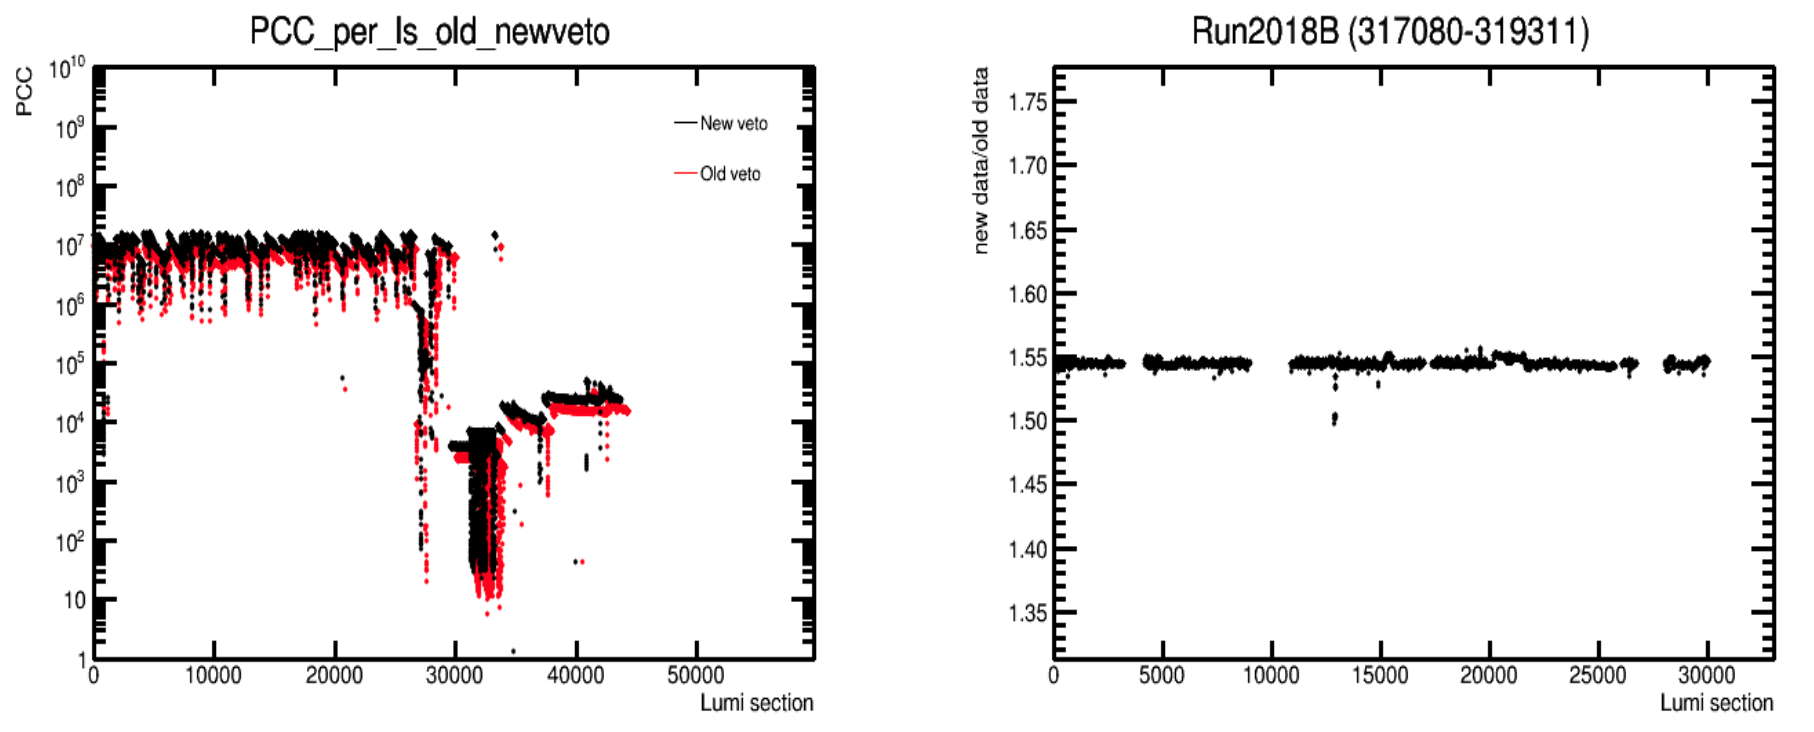
\includegraphics[width=1\textwidth]{ashish_thesis/Run2018B_old_new_veto.png}
\caption{%
    PCC as a function of lumi section for old and new vetolist with its ratio for period B.
}
\label{fig:old_new_veto_B}
\end{figure}


\begin{figure}[!htp]
\centering
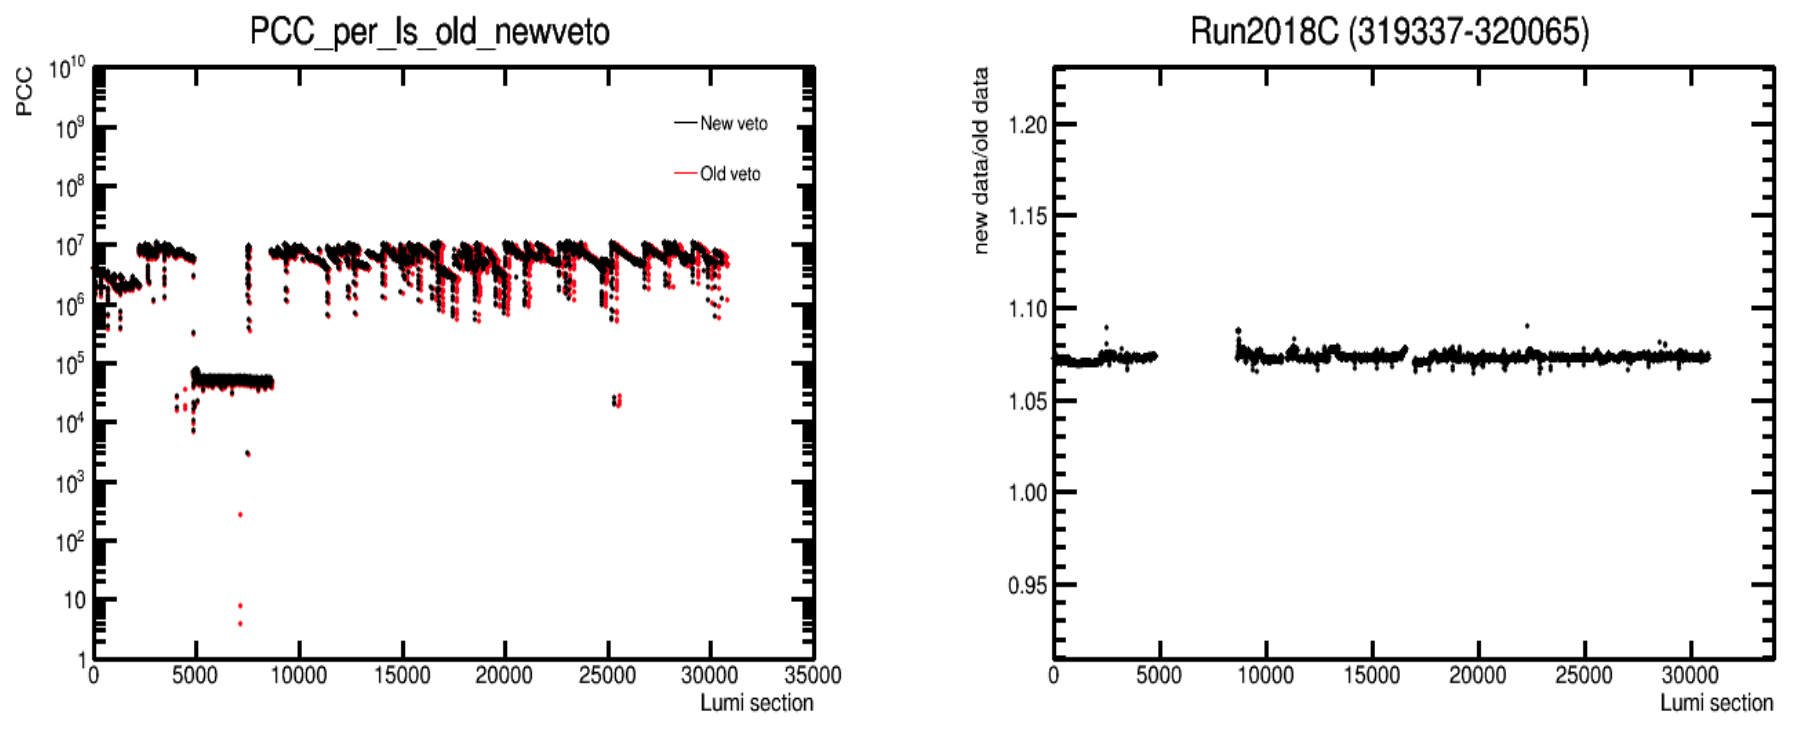
\includegraphics[width=1\textwidth]{ashish_thesis/Run2018C_old_new_veto.png}
\caption{%
    PCC as a function of lumi section for old and new vetolist with its ratio for period C.
}
\label{fig:old_new_veto_C}
\end{figure}


\begin{figure}[!htp]
\centering
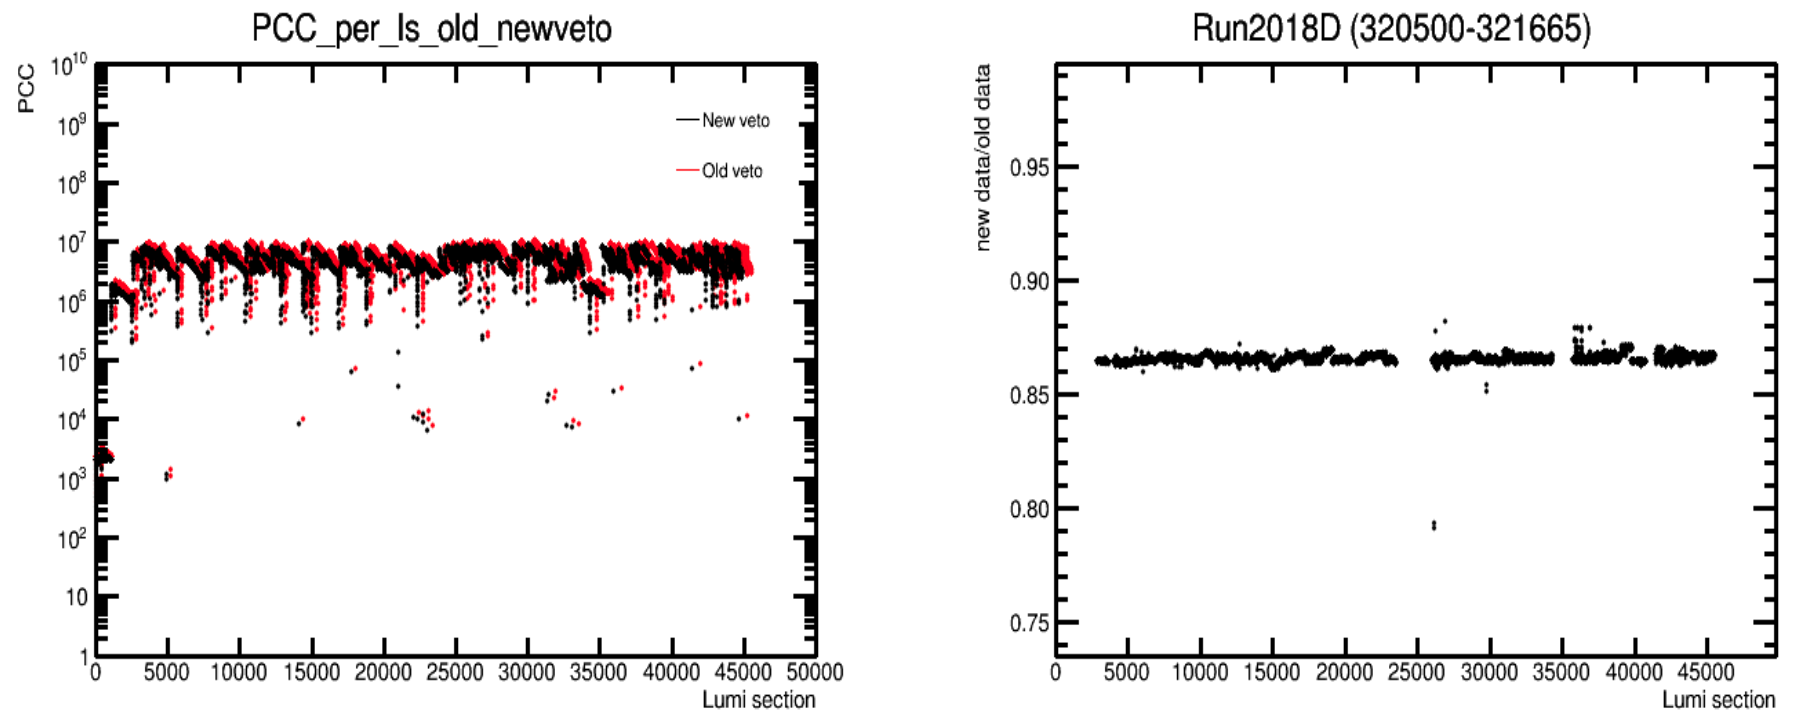
\includegraphics[width=1\textwidth]{ashish_thesis/Run2018D1_old_new_veto.png}
\caption{%
    PCC as a function of lumi section for old and new vetolist with its ratio for period D1.
}
\label{fig:old_new_veto_D1}
\end{figure}

\begin{figure}[!htp]
\centering
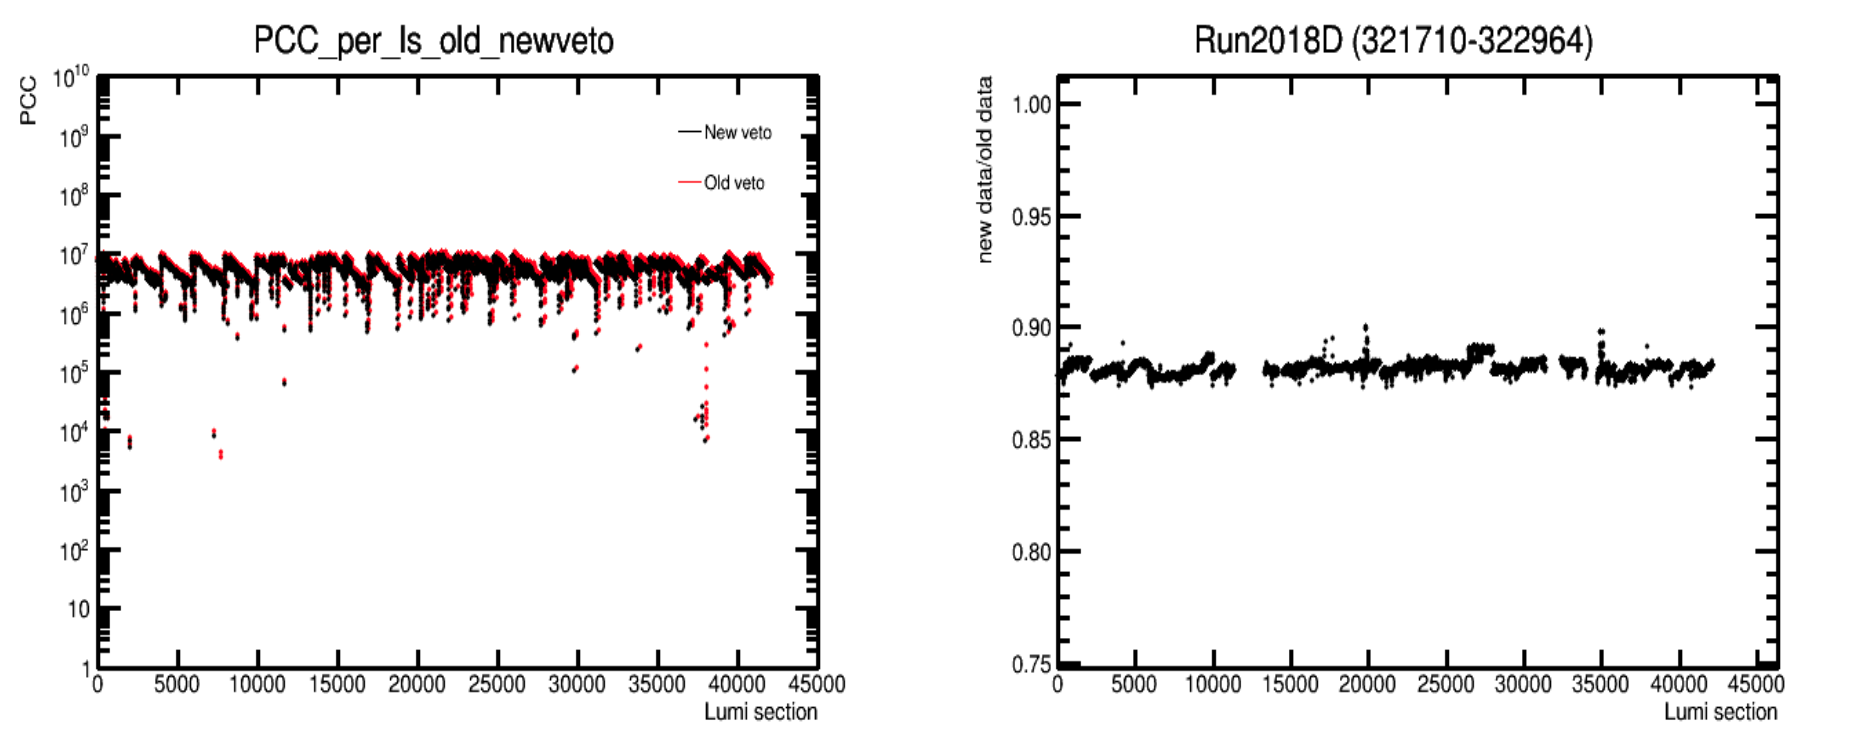
\includegraphics[width=1\textwidth]{ashish_thesis/Run2018D2_old_new_veto.png}
\caption{%
   PCC as a function of lumi section for old and new vetolist with its ratio for period D2.
}
\label{fig:old_new_veto_D2}
\end{figure}

\begin{figure}[!htp]
\centering
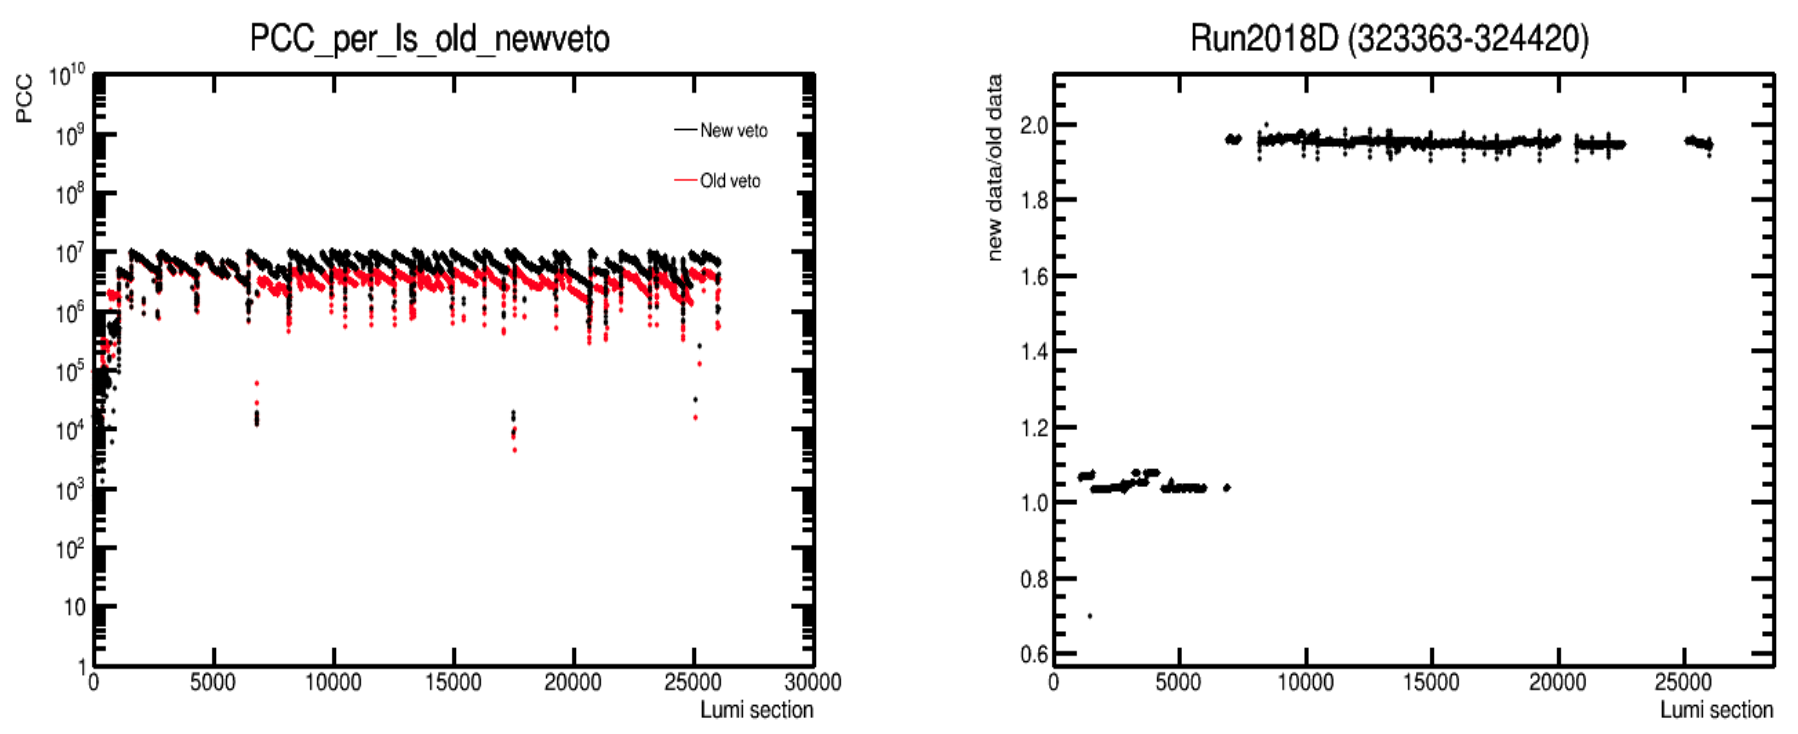
\includegraphics[width=1\textwidth]{ashish_thesis/Run2018D3_old_new_veto.png}
\caption{%
    PCC as a function of lumi section for old and new vetolist with its ratio for period D3.
}
\label{fig:old_new_veto_D3}
\end{figure}

\begin{figure}[!htp]
\centering
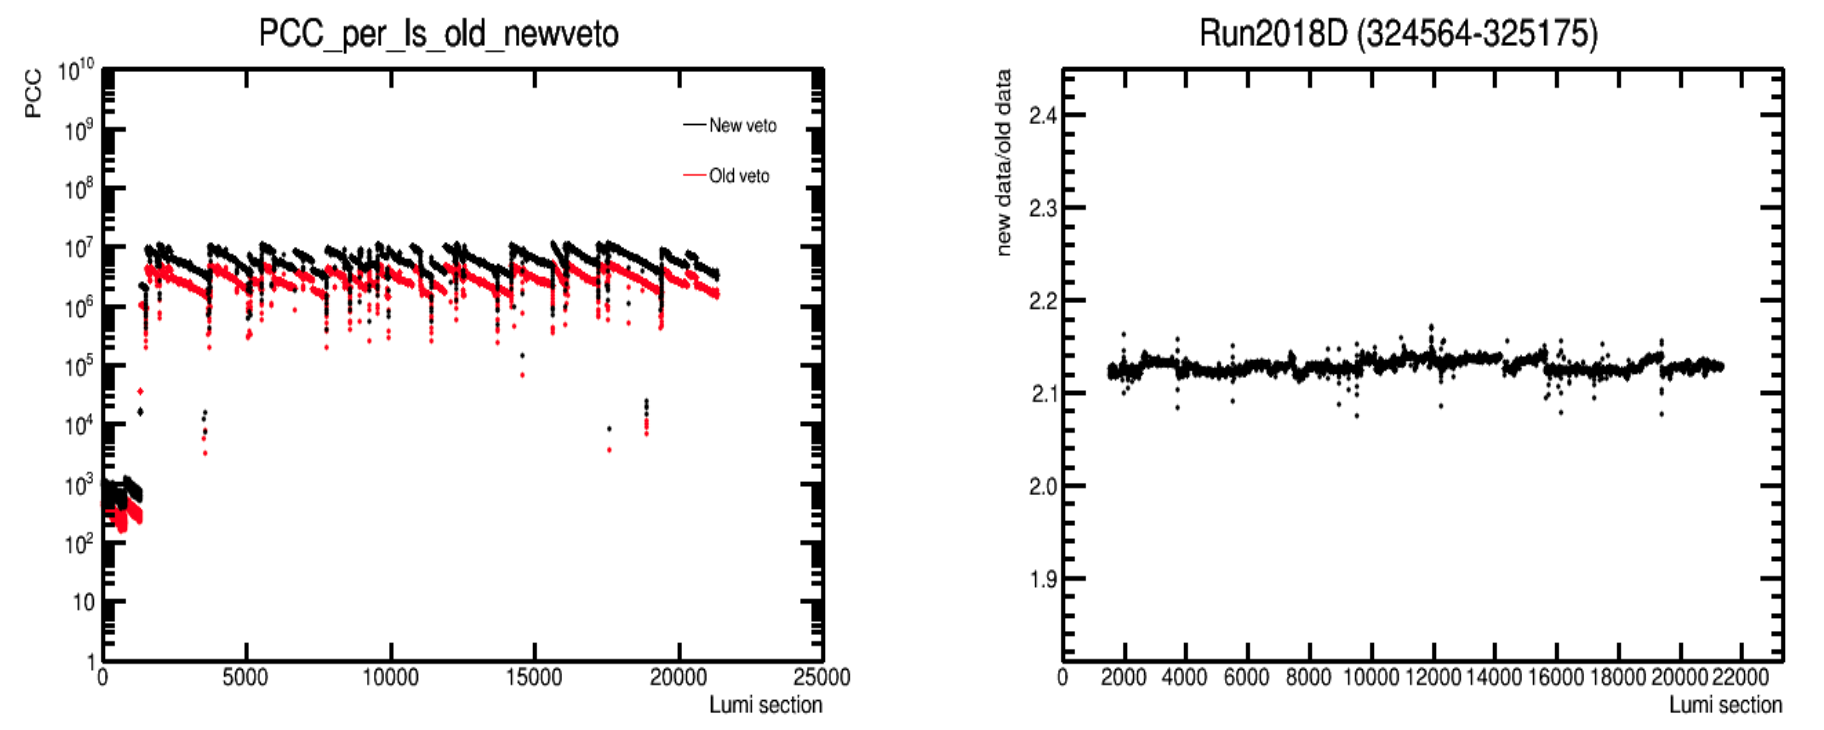
\includegraphics[width=1\textwidth]{ashish_thesis/Run2018D4_old_new_veto.png}
\caption{%
    PCC as a function of lumi section for old and new vetolist with its ratio for period D4.
}
\label{fig:old_new_veto_D3}
\end{figure}

\begin{figure}[!htp]
\centering
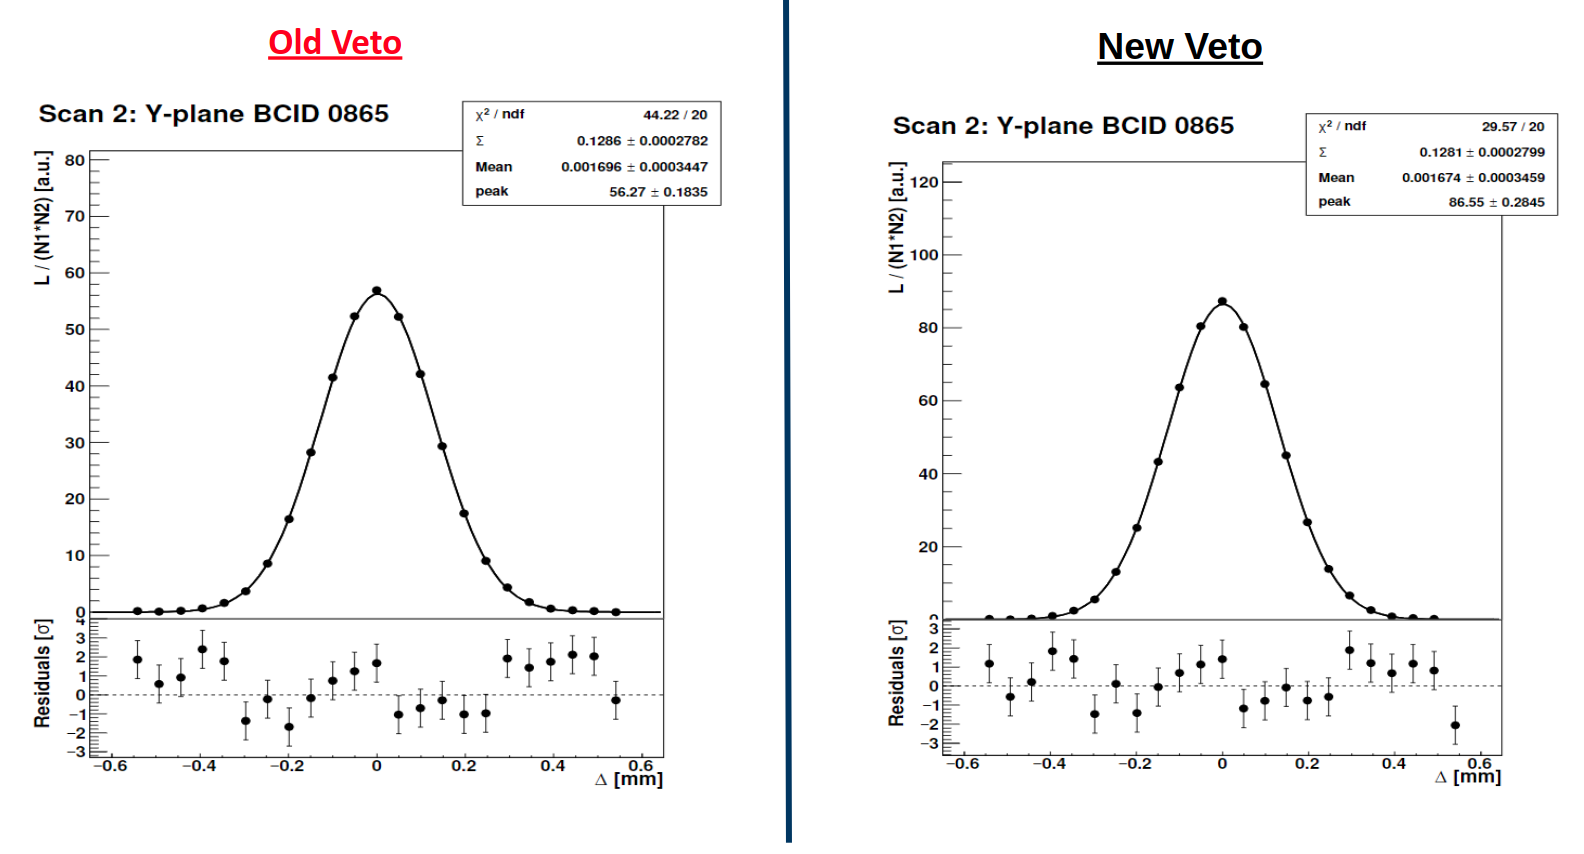
\includegraphics[width=1\textwidth]{ashish_thesis/vdm_fit_old_new_veto.png}
\caption{%
  PCC rate fit for old and new veto.
}
\label{fig:old_new_veto_vdmfit}
\end{figure}


\begin{figure}[!htp]
\centering
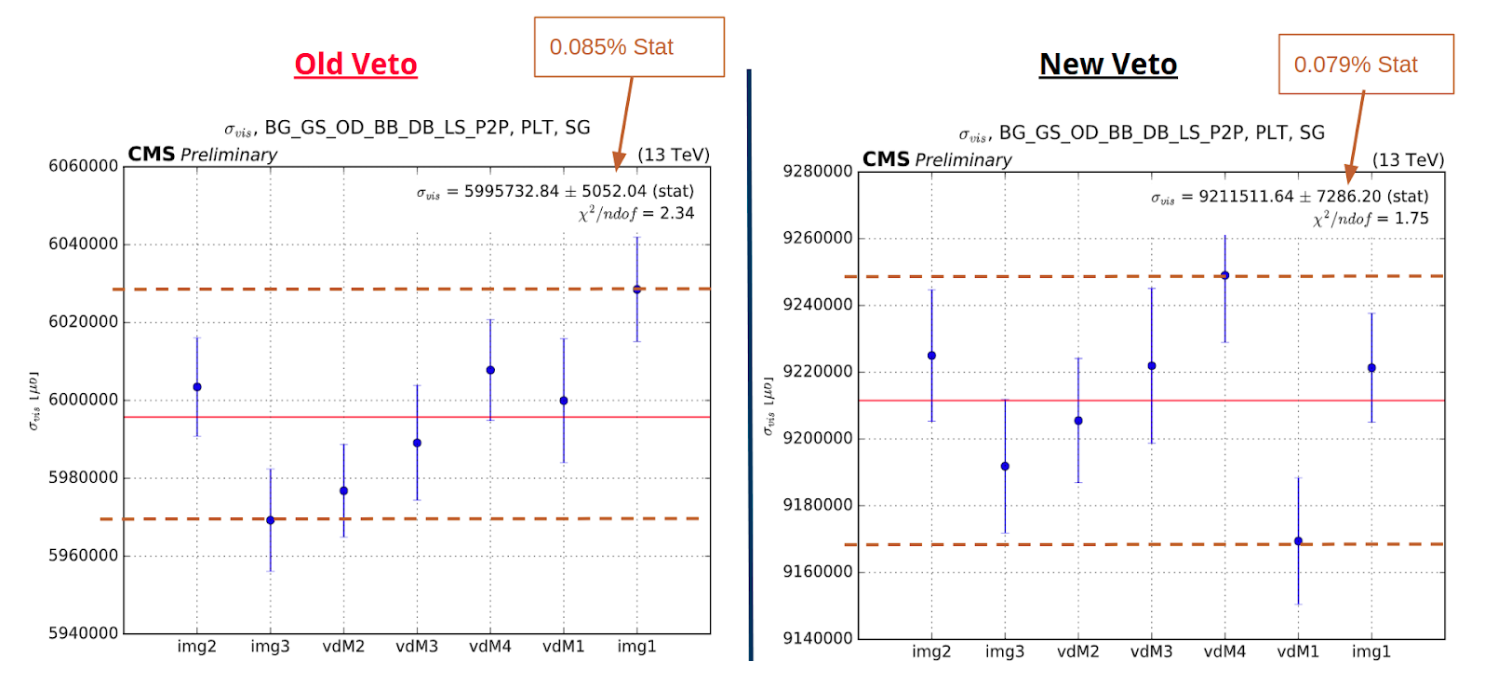
\includegraphics[width=1\textwidth]{ashish_thesis/sigmavis_old_new_veto.png}
\caption{%
   PCC visible cross section averaged over bunch ids for each scan for old and new veto.
}
\label{fig:old_new_veto_sigmavis}
\end{figure}


\begin{figure}[!htp]
\centering
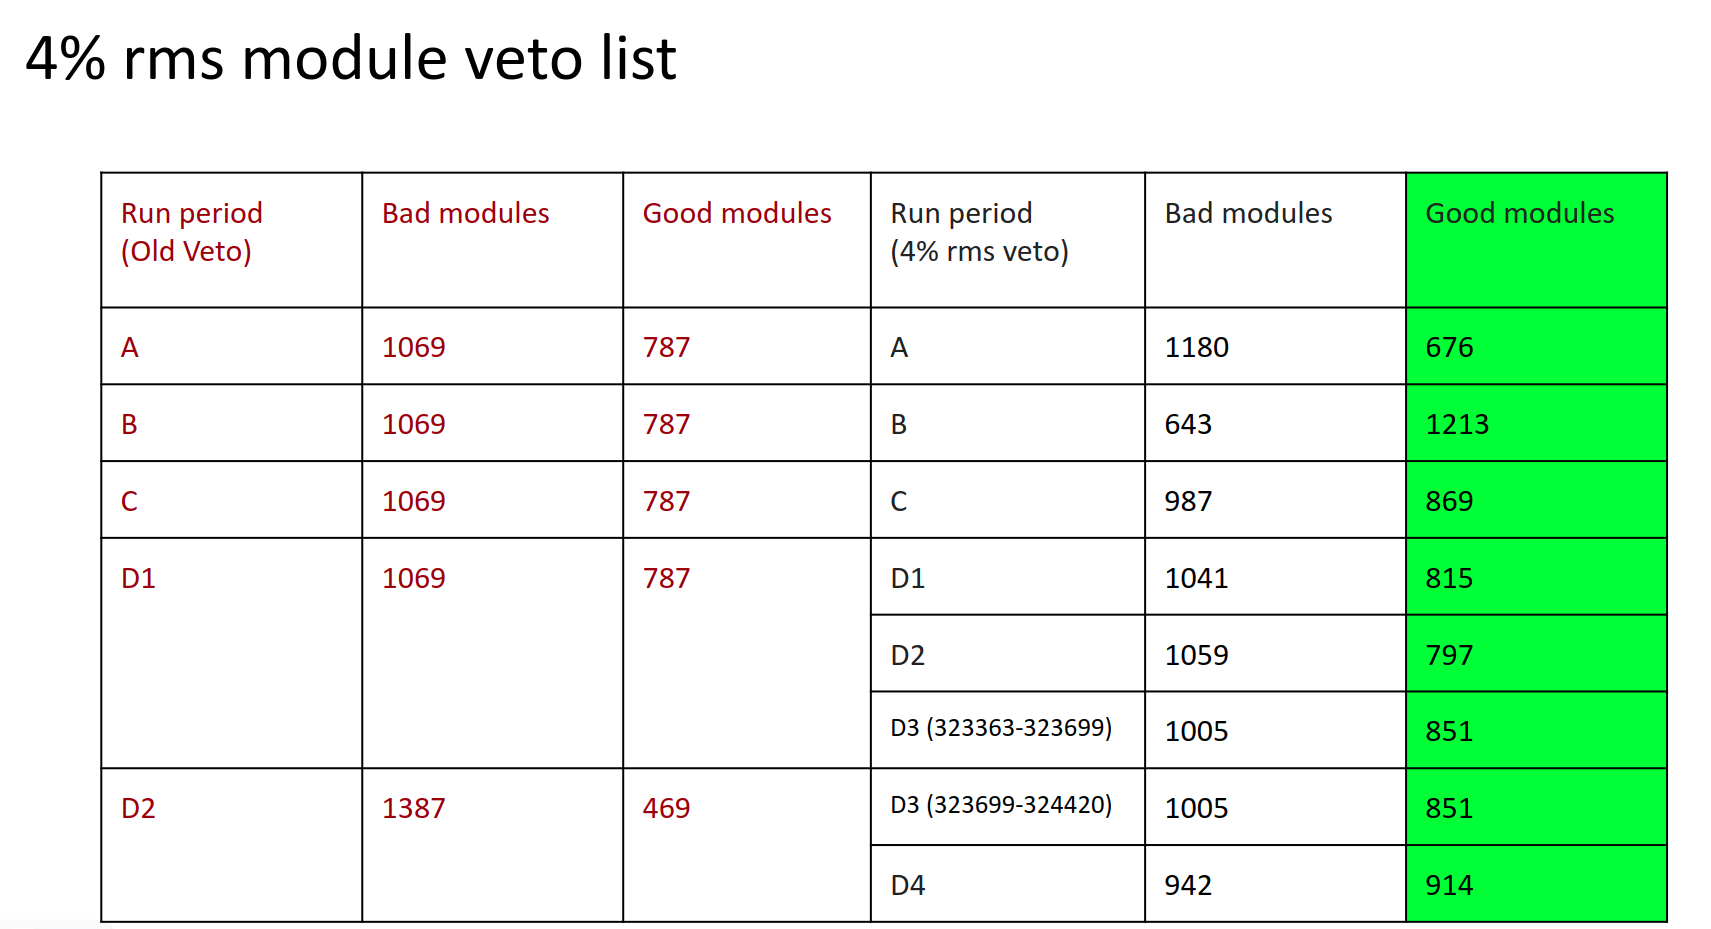
\includegraphics[width=1\textwidth]{ashish_thesis/4per_rms_veto.png}
\caption{%
   klm
}
\label{fig:4per_veto}
\end{figure}


\begin{figure}[!htp]
\centering
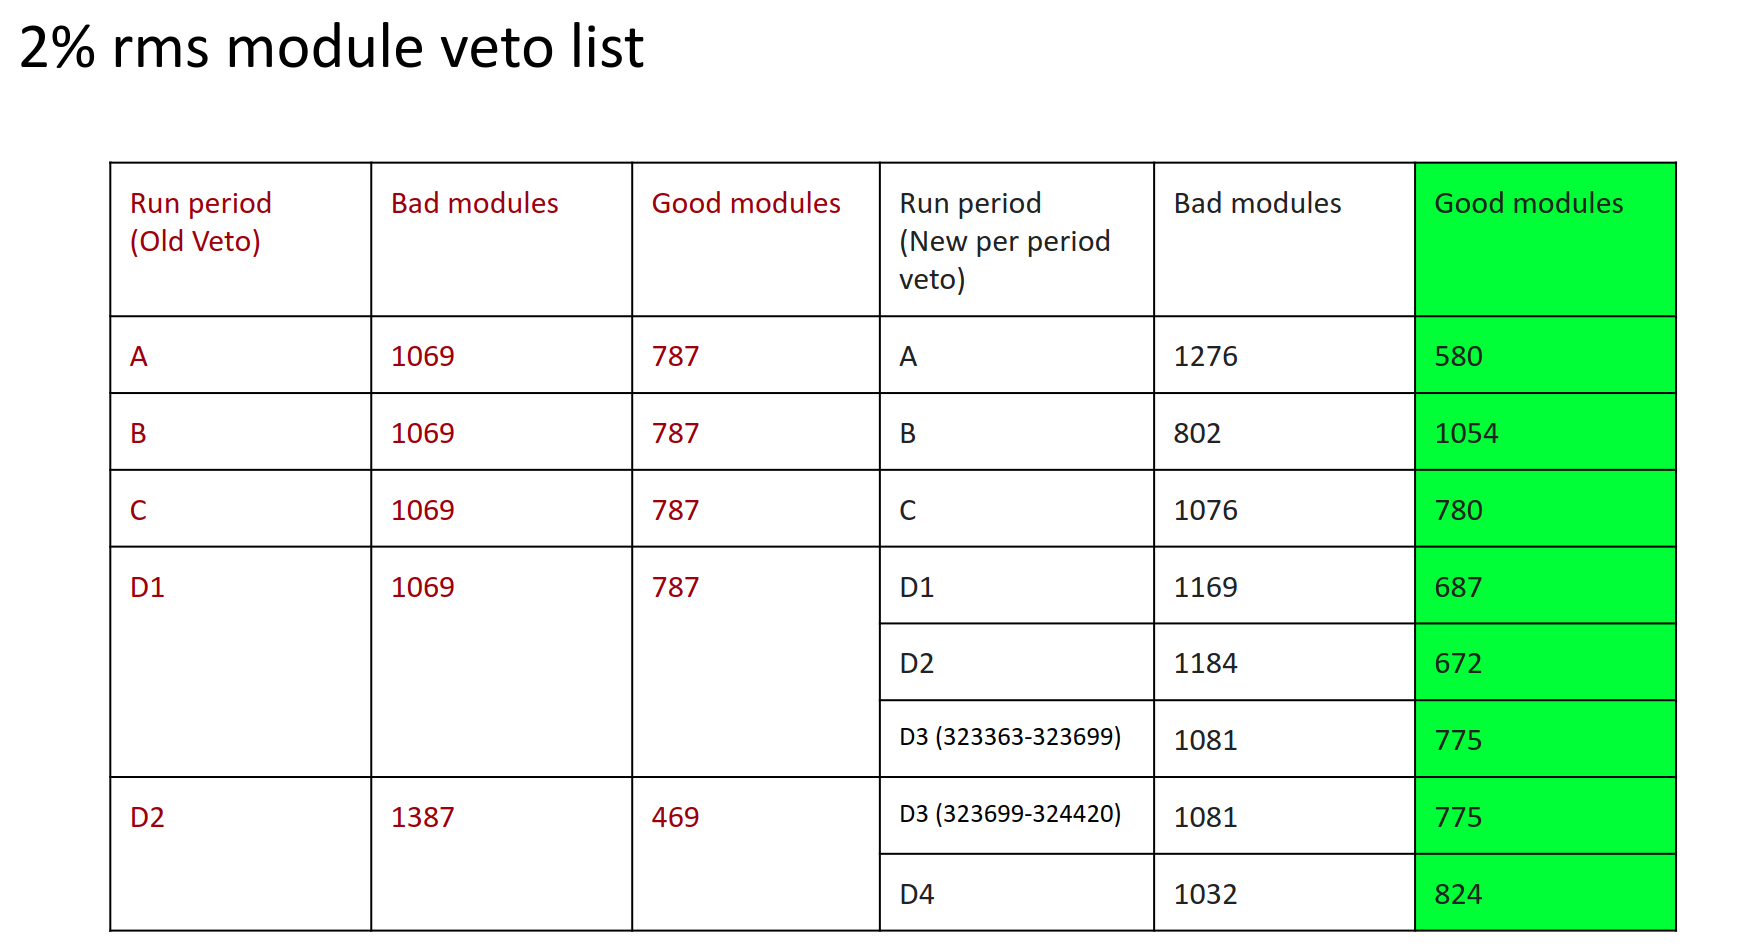
\includegraphics[width=1\textwidth]{ashish_thesis/2per_rms_veto.png}
\caption{%
   X and Y plane vdM fit for BCID 0865 using 2\% rms  vetolist.
}
\label{fig:2per_veto}
\end{figure}


\begin{figure}[!htp]
\centering
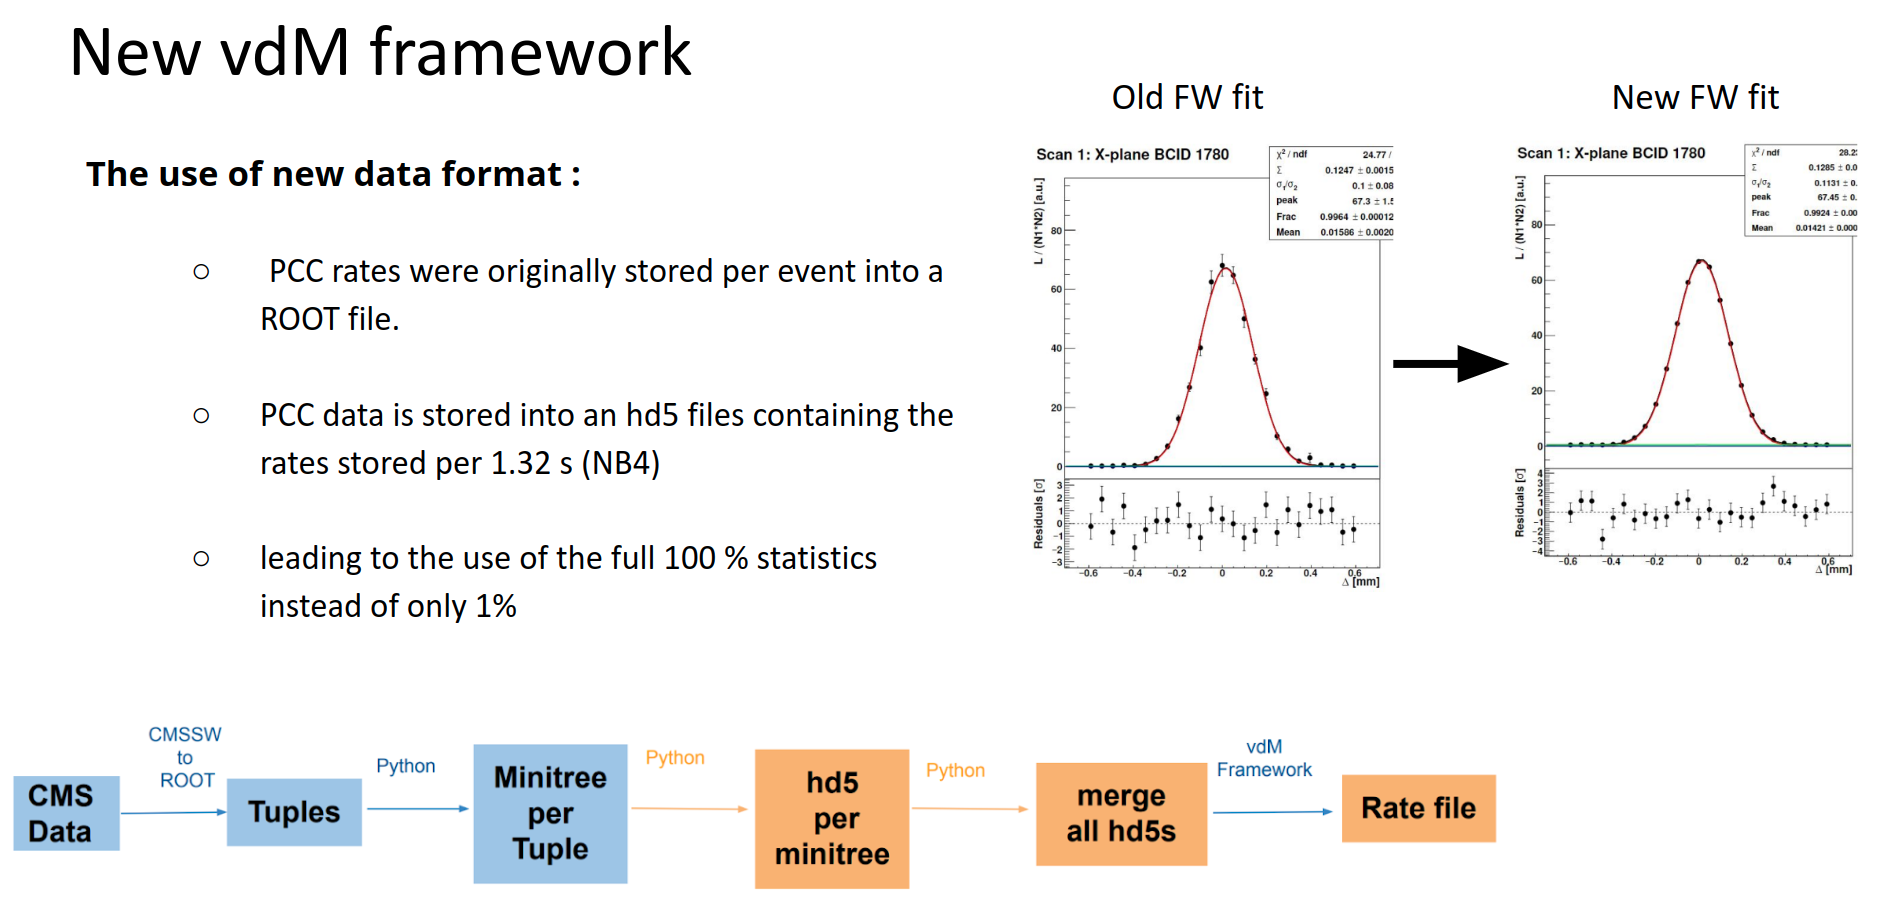
\includegraphics[width=1\textwidth]{ashish_thesis/new_framework_vdm.png}
\caption{%
   klm
}
\label{fig:vdm_new_f}
\end{figure}



\begin{figure}[!htp]
\centering
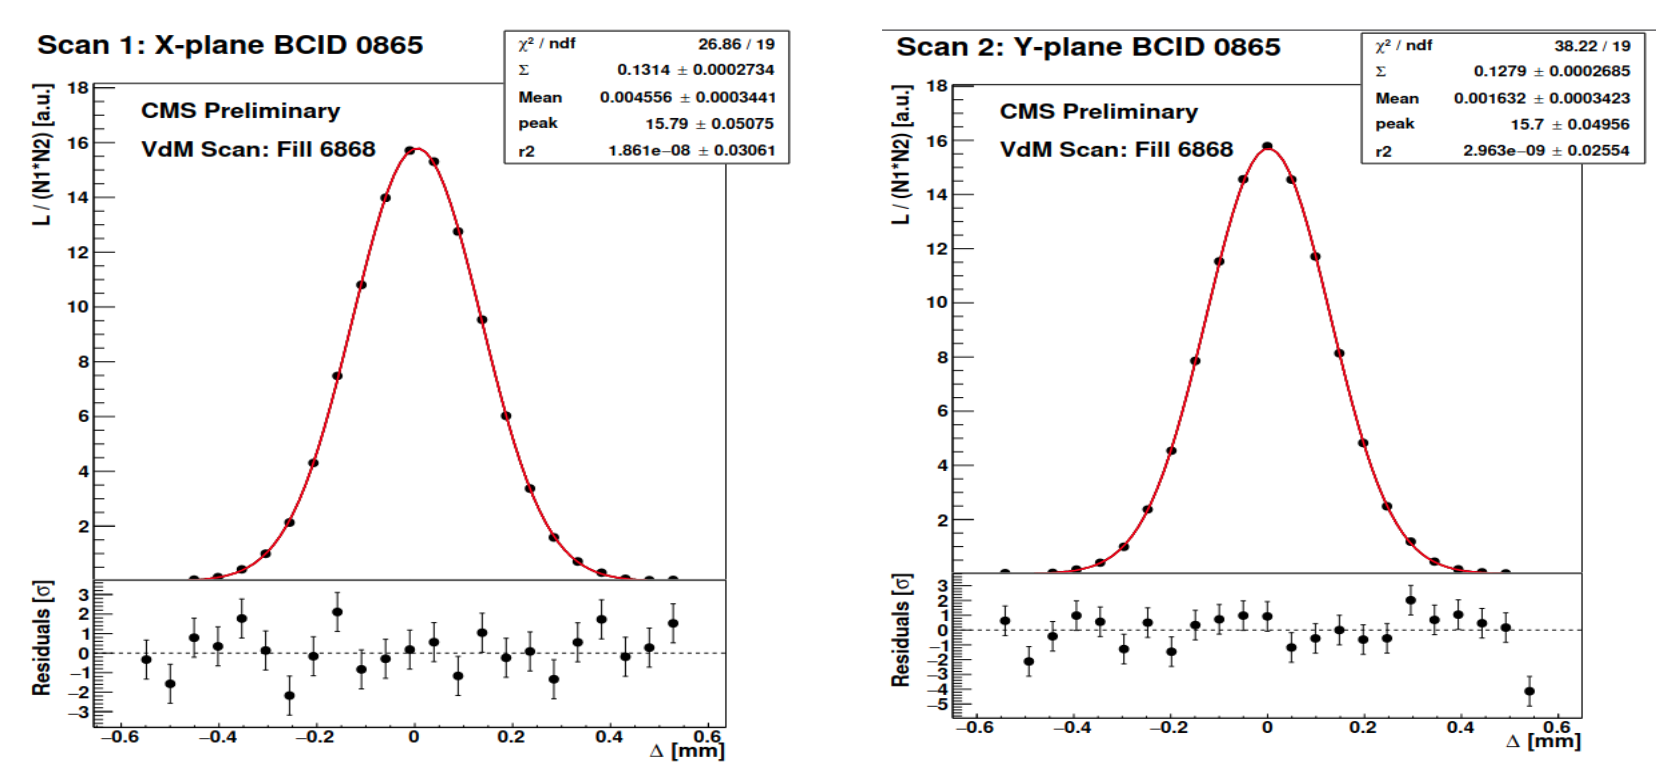
\includegraphics[width=1\textwidth]{ashish_thesis/vdm_fit_4per_rms_veto.png}
\caption{%
   vdM fit for 4\% rms common module vetolist.
}
\label{fig:vdm_fit_4rms}
\end{figure}



%\begin{comment}


\begin{figure}[!htp]
\centering
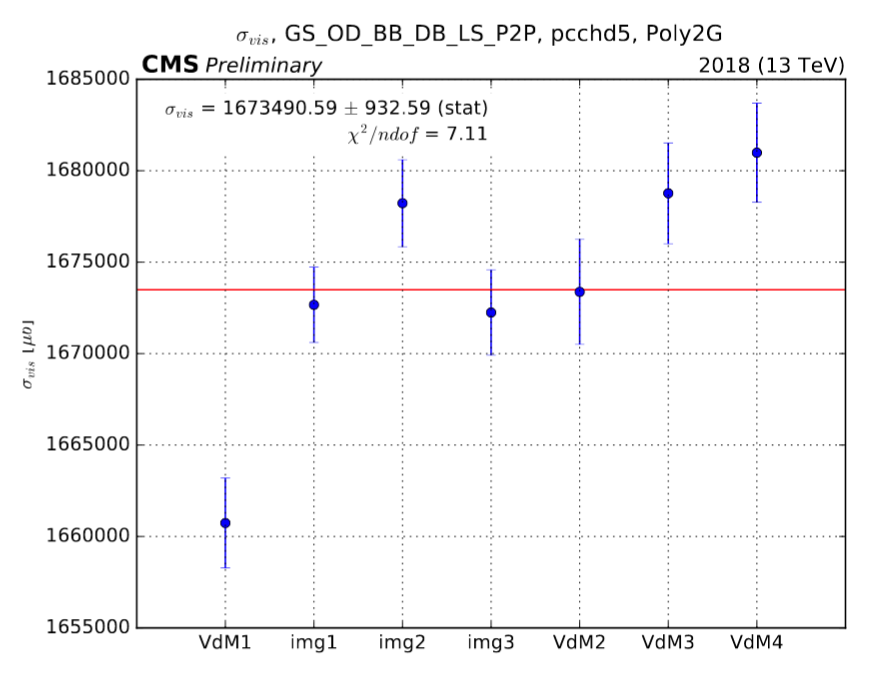
\includegraphics[width=0.7\textwidth]{ashish_thesis/sigmavis_4per_rms.png}
\caption{%
   PCC visible cross section for 4 percent rms common vetolist.
}
\label{fig:sigmavis_4rms}
\end{figure}


\begin{figure}[!htp]
\centering
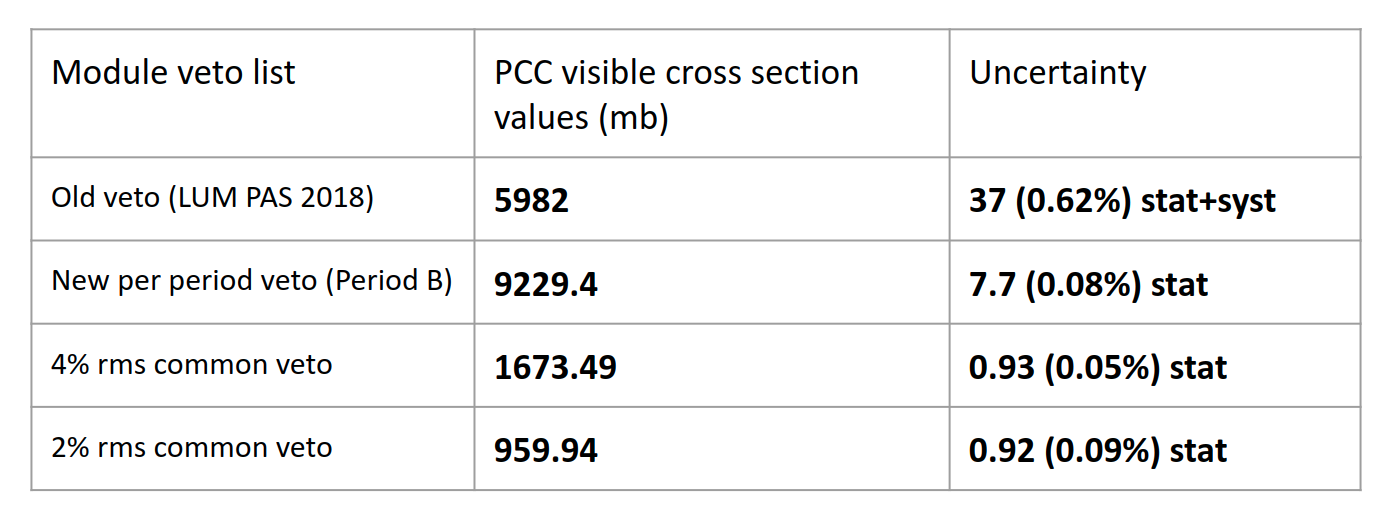
\includegraphics[width=1\textwidth]{ashish_thesis/sigmavis_diff_veto.png}
\caption{%
   klm
}
\label{fig:sigmavis_diff_veto}
\end{figure}

\begin{table}[!ht]
\centering
\topcaption{%
    pcc visible cross section for different module vetolist.
}
\begin{tabular}{ccccc}
    \textbf{Module veto list} & \textbf{PCC visible cross section values (mb)} & \textbf{Uncertainty} \\ \hline
    Old veto (LUM PAS 2018) & 5982 & 37 (0.08\%) stat+syst \\
    New per period veto (Period B) & 9229.4  & 7.7 (0.08\%) stat \\
    4\% rms common veto & 1673.49  & 0.93 (0.05\%) stat \\
    2\% rms common veto & 959.94  & 0.92 (0.09\%) stst \\
\end{tabular}
\label{tab:pccvis_diffveto}
\end{table}



\begin{figure}[!htp]
\centering
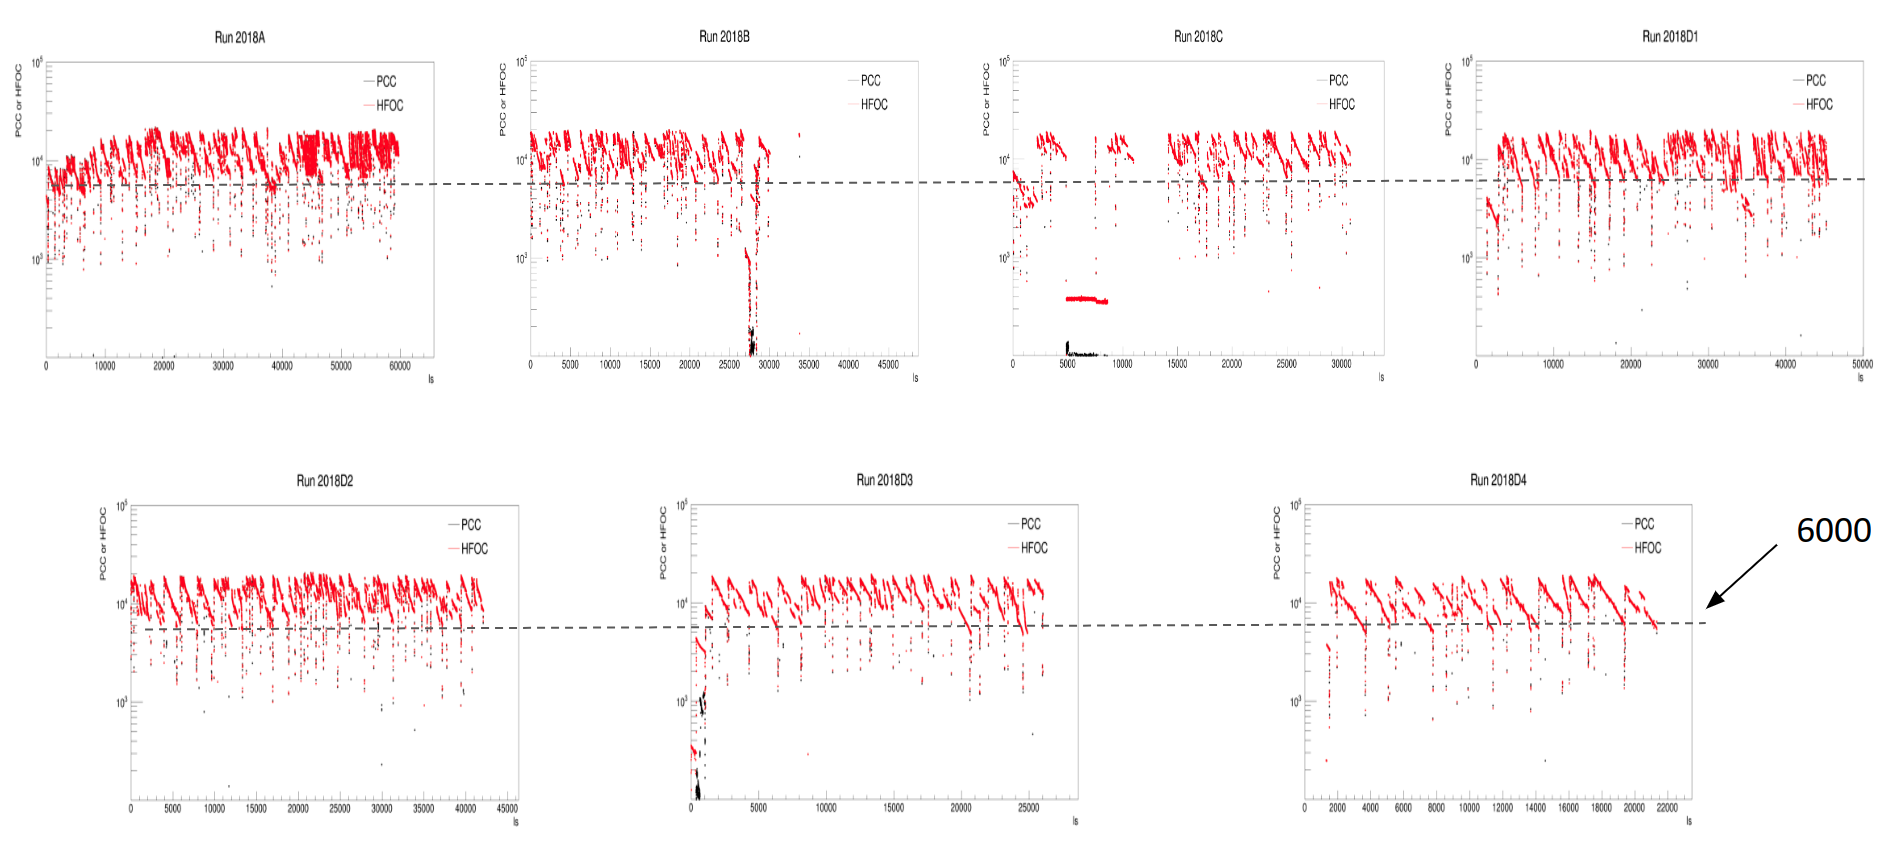
\includegraphics[width=1\textwidth]{ashish_thesis/sys_unc_totPCC_cut.png}
\caption{%
   Selection on total PCC to remove low statistics lumi section for all period.
}
\label{fig:totpcccut_sys_unc}
\end{figure}



\begin{figure}[!htp]
\centering
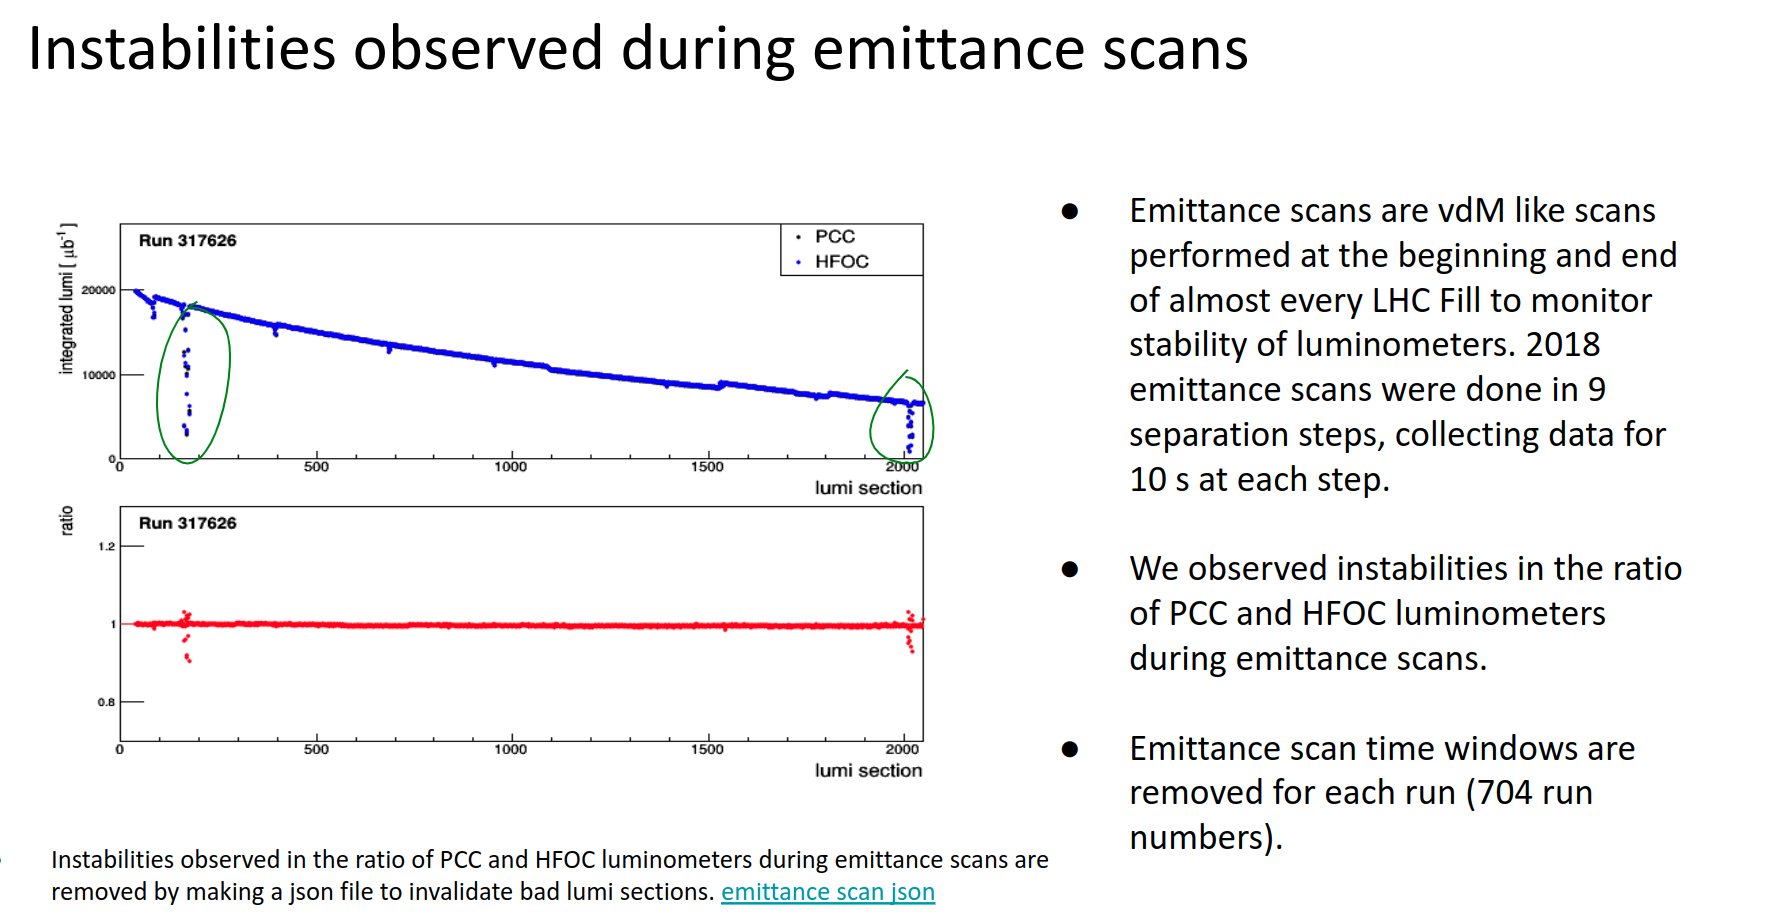
\includegraphics[width=1\textwidth]{ashish_thesis/emittance_scans.png}
\caption{%
   Emittance scans are vdM like scans performed at the beginning and end of almost every LHC Fill to monitor stability of luminometers. 2018 emittance scans were done in 9 separation steps, collecting data for 10 s at each step. We observed instabilities in the ratio of PCC and HFOC luminometers during emittance scans. 
}
\label{fig:emitscan}
\end{figure}


\begin{figure}[!htp]
\centering
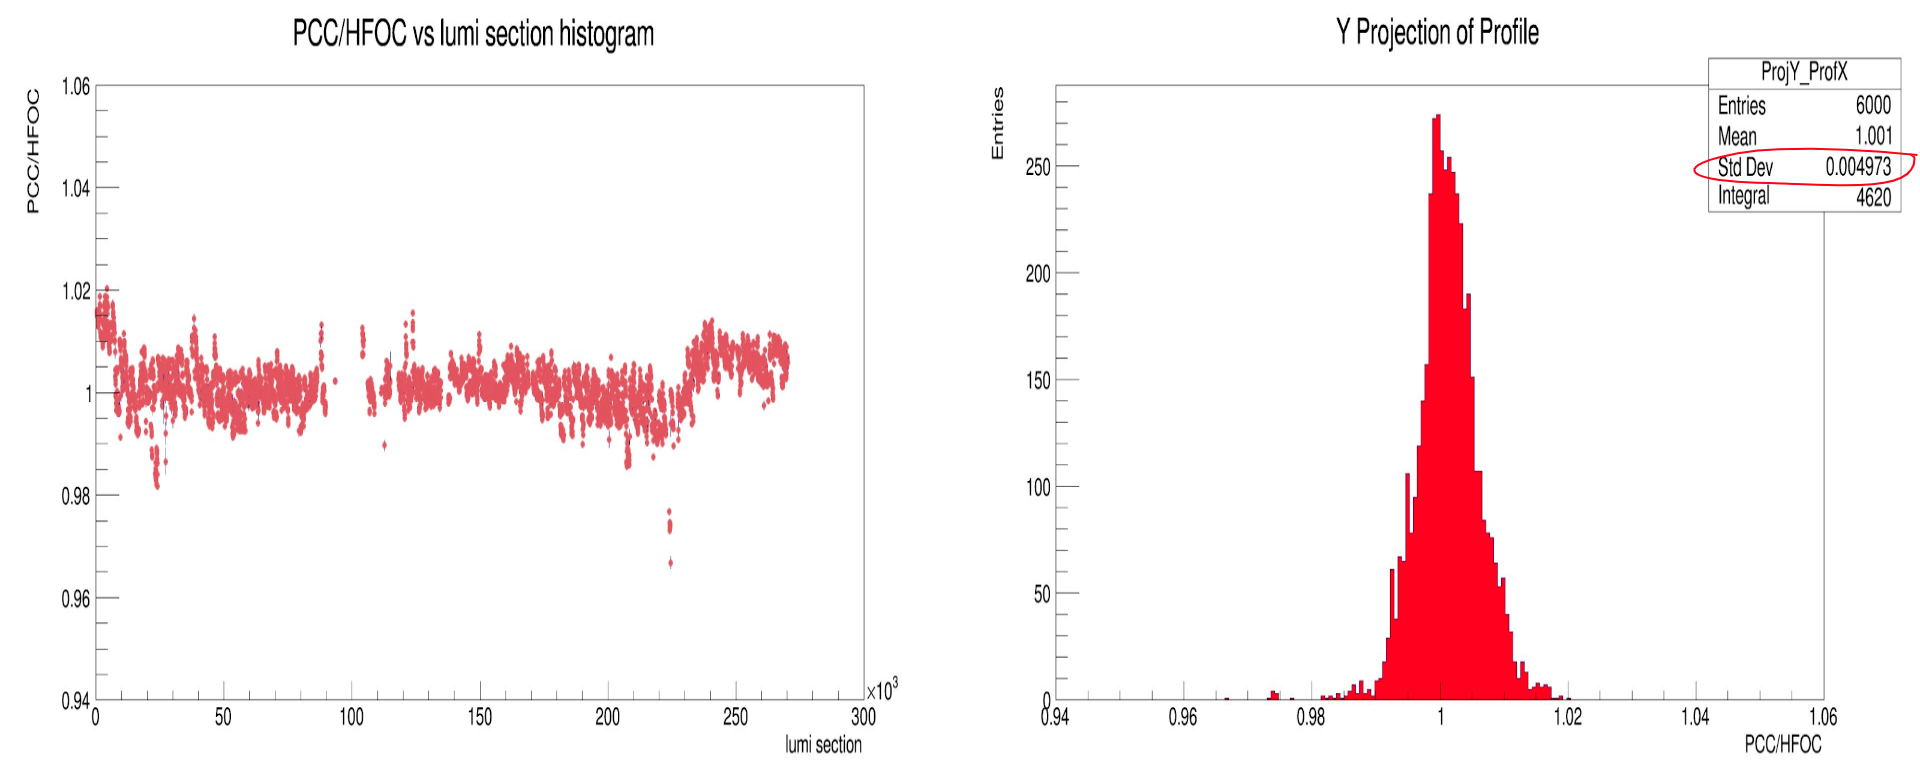
\includegraphics[width=1\textwidth]{ashish_thesis/pcc_hfoc_ratio_stability_old_veto.png}
\caption{%
   Left: X profile of PCC/HFOC luminosity ratio as a function of lumi section for old veto showing instabilities.  Right: Y projection of the X profile of the luminosity ratio. The standard deviation of this projection is taken as the systematic uncertainty due to stability.
}
\label{fig:pcc_hfoc_old}
\end{figure}

\begin{figure}[!htp]
\centering
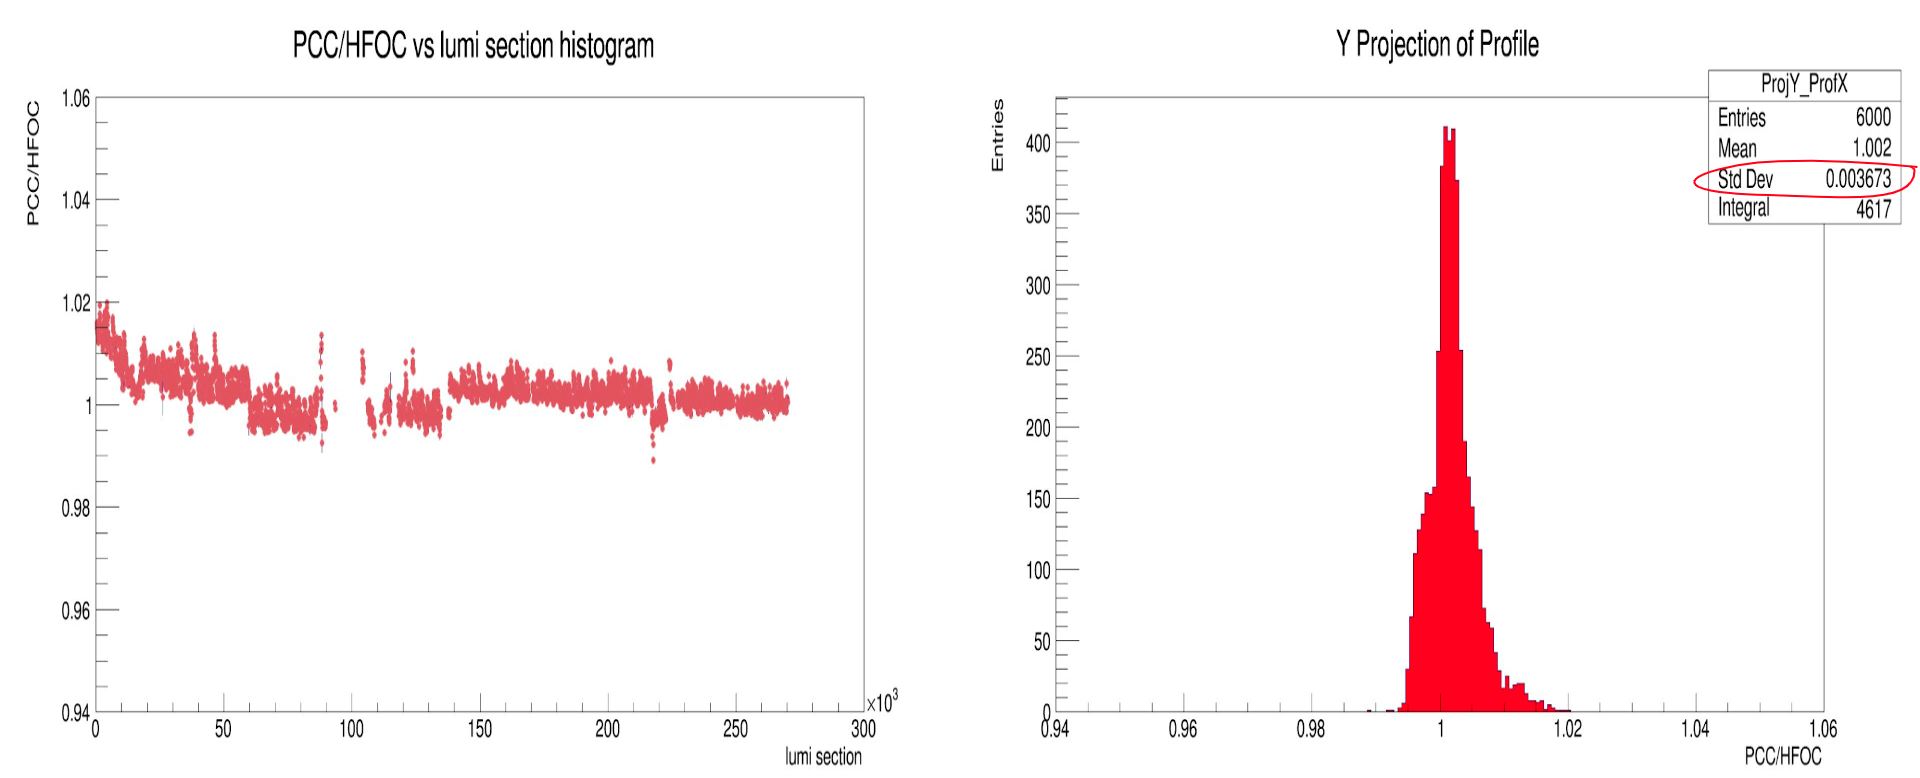
\includegraphics[width=1\textwidth]{ashish_thesis/pcc_hfoc_ratio_stability_new_veto.png}
\caption{%
  Left: X profile of PCC/HFOC luminosity ratio as a function of lumi section for new veto showing instabilities.  Right: Y projection of the X profile of the luminosity ratio. The standard deviation of this projection is taken as the systematic uncertainty due to stability.
}
\label{fig:pcc_hfoc_new}
\end{figure}

\begin{figure}[!htp]
\centering
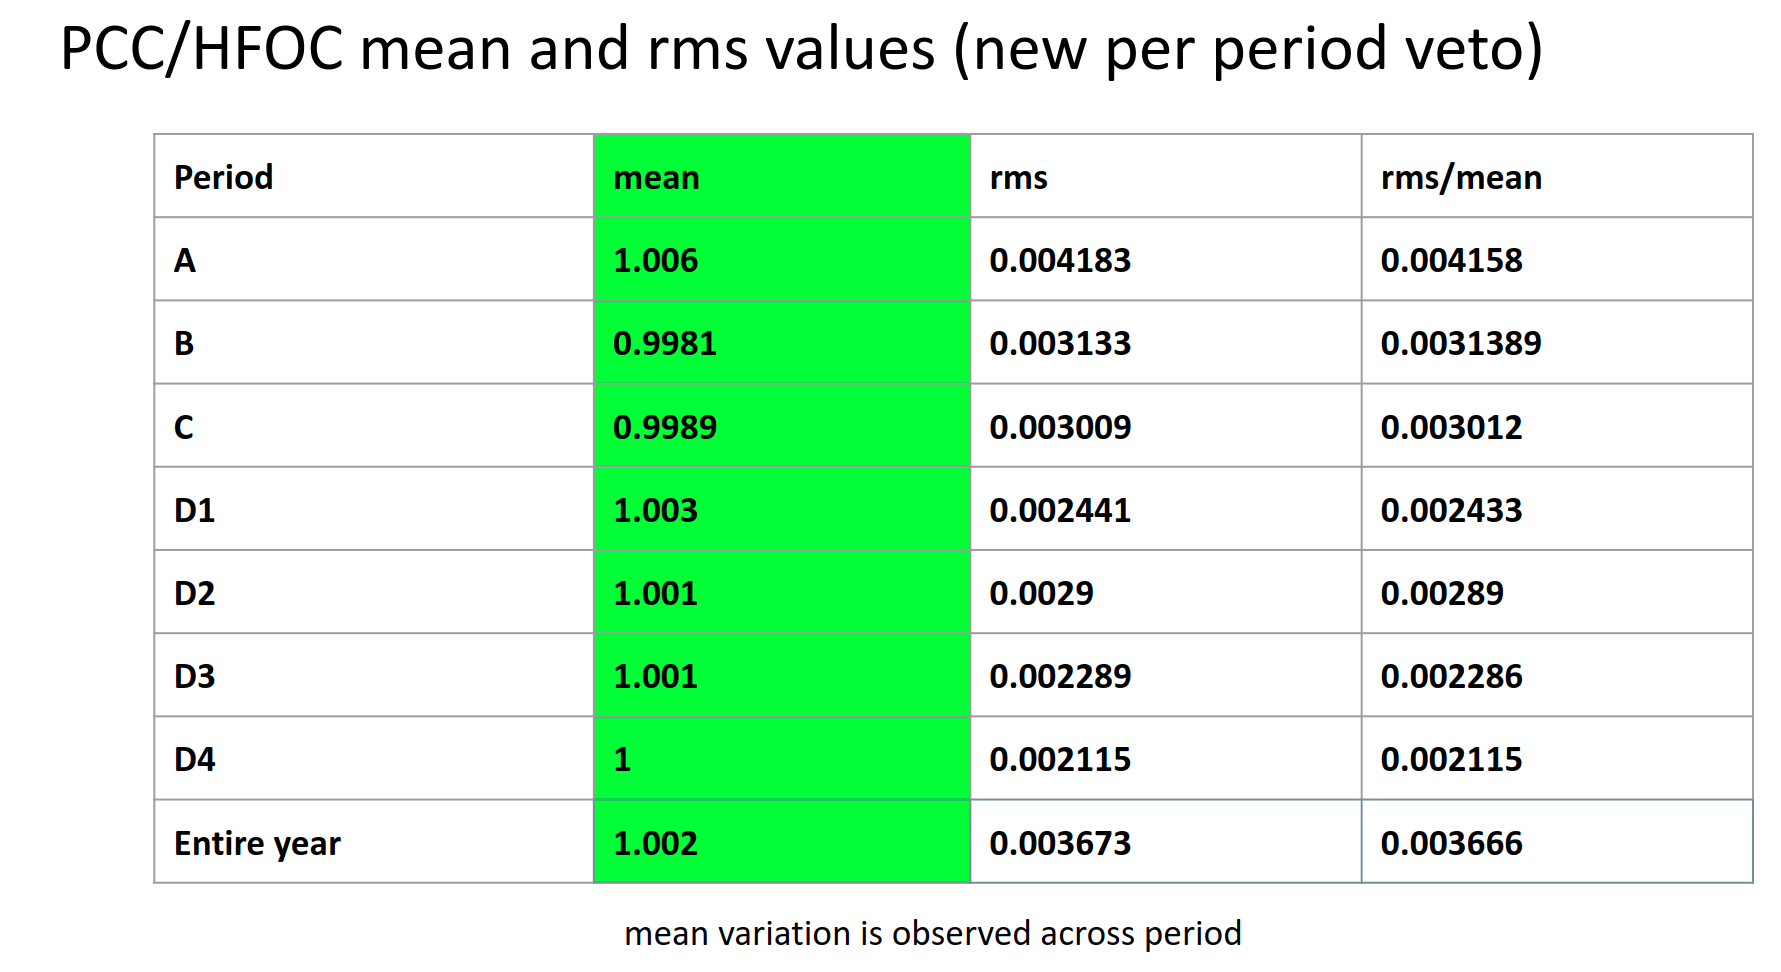
\includegraphics[width=1\textwidth]{ashish_thesis/pcc_hfoc_mean_rms_periods_new_veto.png}
\caption{%
   
}
\label{fig:pcc_hfoc_new_mean_rms}
\end{figure}



\begin{table}[!ht]
\centering
\topcaption{%
    PCC/ HFOC luminosity mean and rms values for new per period vetolist showing variation in mean values across period.
}
\begin{tabular}{ccccc}
    \textbf{Period} & \textbf{mean} & \textbf{rms} &  \textbf{rms/mean} \\ \hline
    A & 1.006 & 0.004183 & 0.004158 \\
    B & 0.9981  & 0.003133 & 0.0031389 \\
    C & 0.9989  & 0.003009 & 0.003012\\
    D1 & 1.003  & 0.002441 & 0.002433 \\
    D2 & 1.001  & 0.0029 & 0.00289 \\
   D3  & 1  & 0.002115 & 0.002115 \\
   D4  & 1.002  & 0.003673 & 0.003666 \\ 
\end{tabular}
\label{tab:pccvis_diffveto}
\end{table}



\begin{figure}[!htp]
\centering
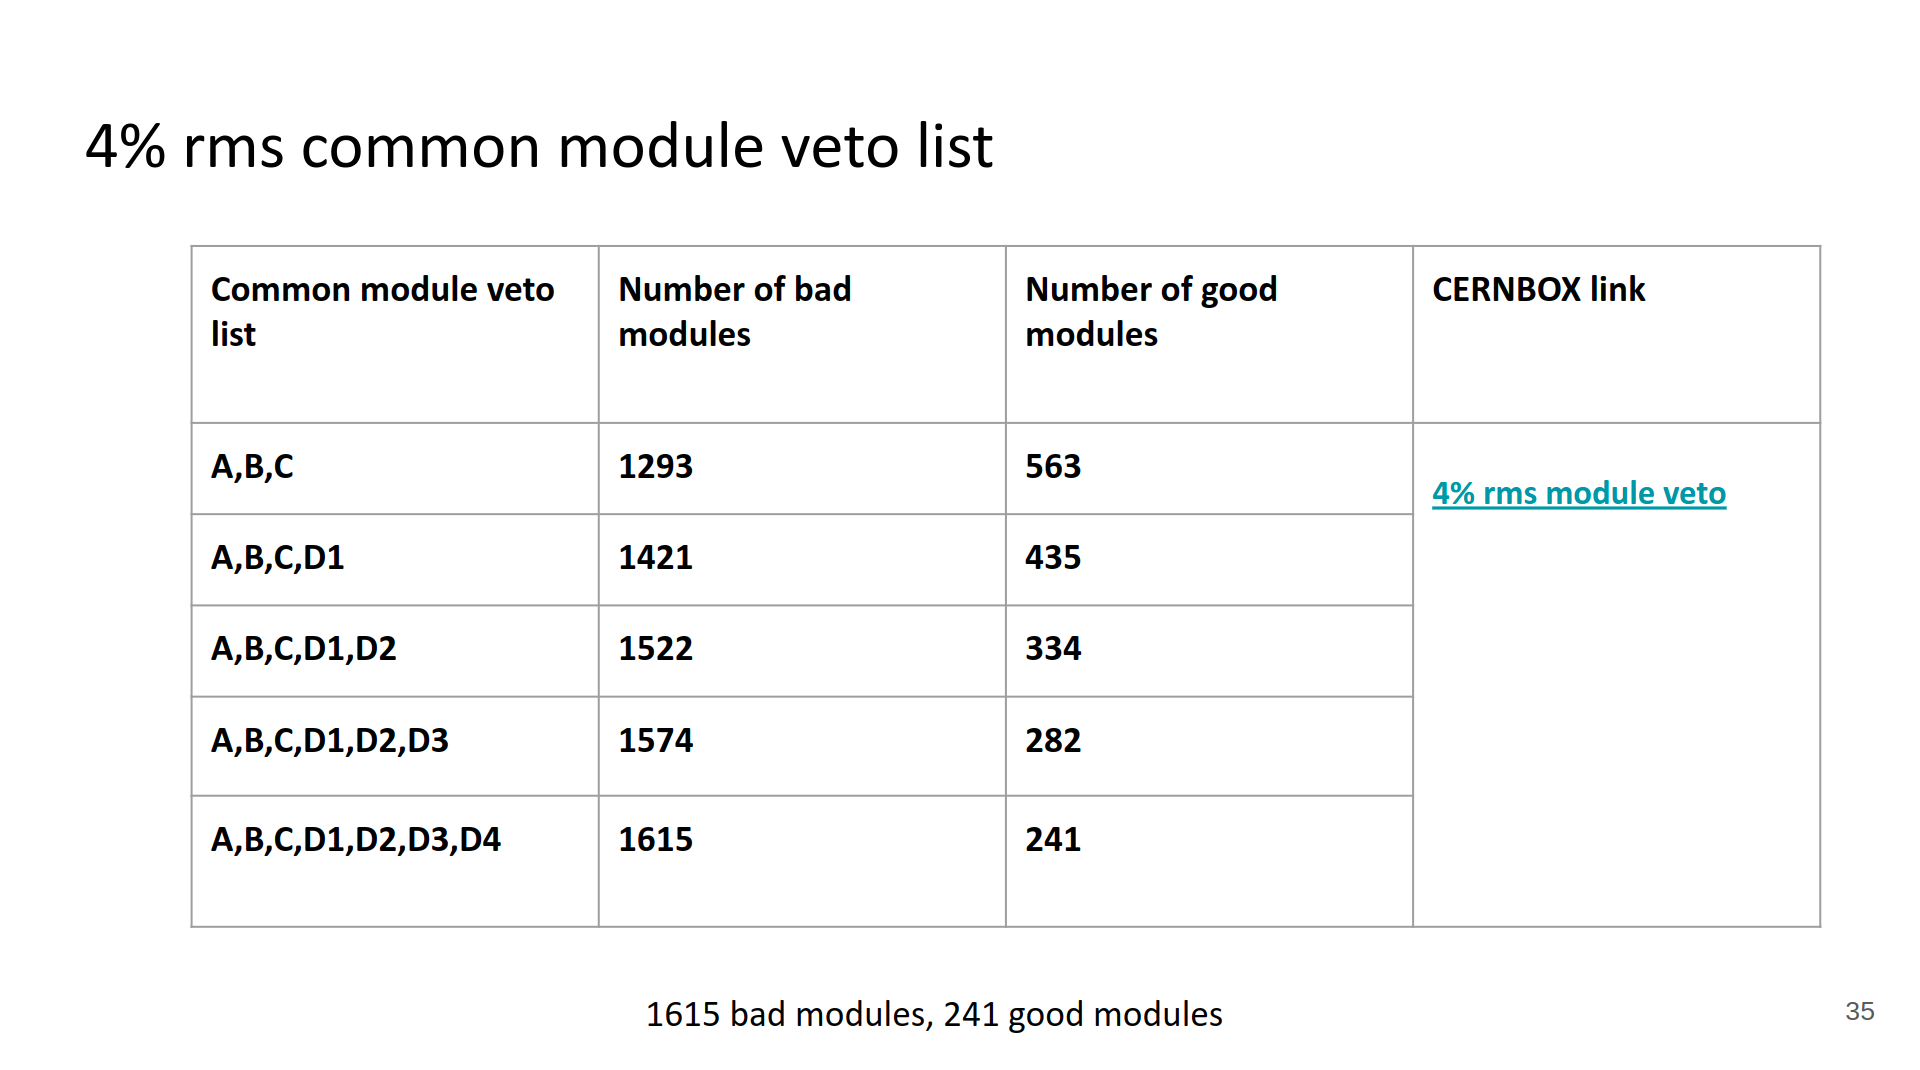
\includegraphics[width=1\textwidth]{ashish_thesis/4per_rms_common_veto.png}
\caption{%
   4 per common veto
}
\label{fig:4per common veto}
\end{figure}


\begin{table}[!ht]
\centering
\topcaption{%
    A method to make 4\% rms commpon module vetolist.
}
\begin{tabular}{ccccc}
    \textbf{Common module vetolist} & \textbf{# bad modules} & \textbf{# good modules} \\ \hline
    A, B, C & 1293 & 563  \\
    A, B, C, D1 & 1421  & 435  \\
    A, B, C, D1, D2 & 1522  & 334 \\
    A, B, C, D1, D2, D3 & 1574  & 282  \\
   A, B, C, D1, D2, D3, D4  & 1615  & 241 \\
\end{tabular}
\label{tab:pccvis_diffveto}
\end{table}






\begin{figure}[!htp]
\centering
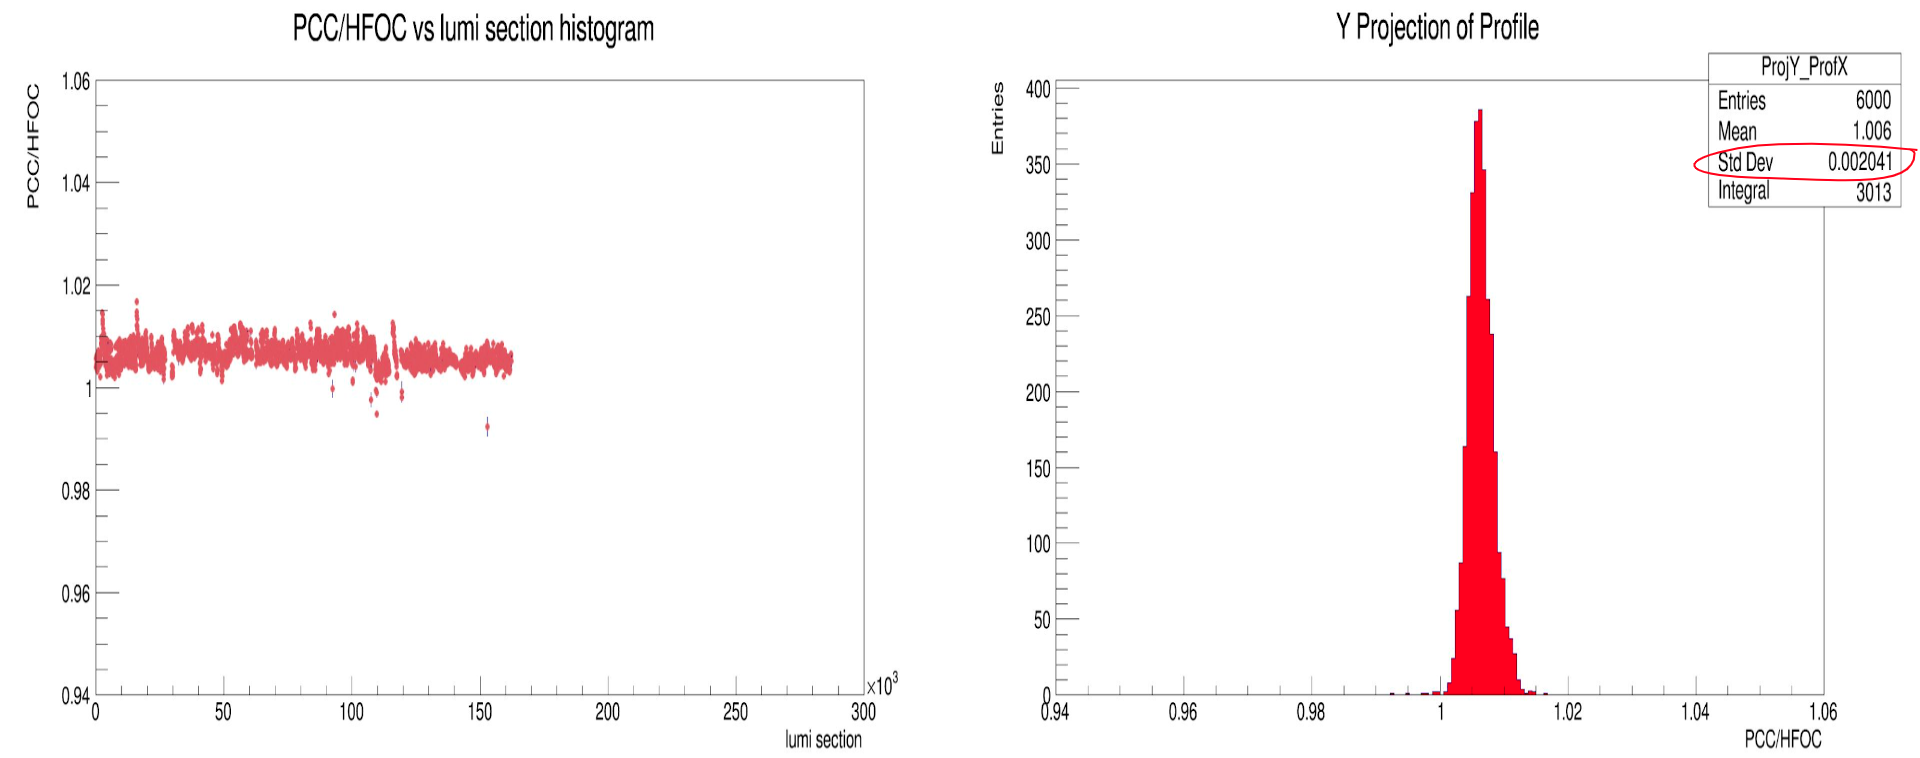
\includegraphics[width=1\textwidth]{ashish_thesis/pcc_hfoc_ratio_stability_4per_common_veto.png}
\caption{%
   Left: X profile of PCC/HFOC luminosity ratio as a function of lumi section for 4\% rms commpon module veto showing instabilities.  Right: Y projection of the X profile of the luminosity ratio. The standard deviation of this projection is taken as the systematic uncertainty due to stability.
}
\label{fig:4per common veto sys}
\end{figure}



\begin{figure}[!htp]
\centering
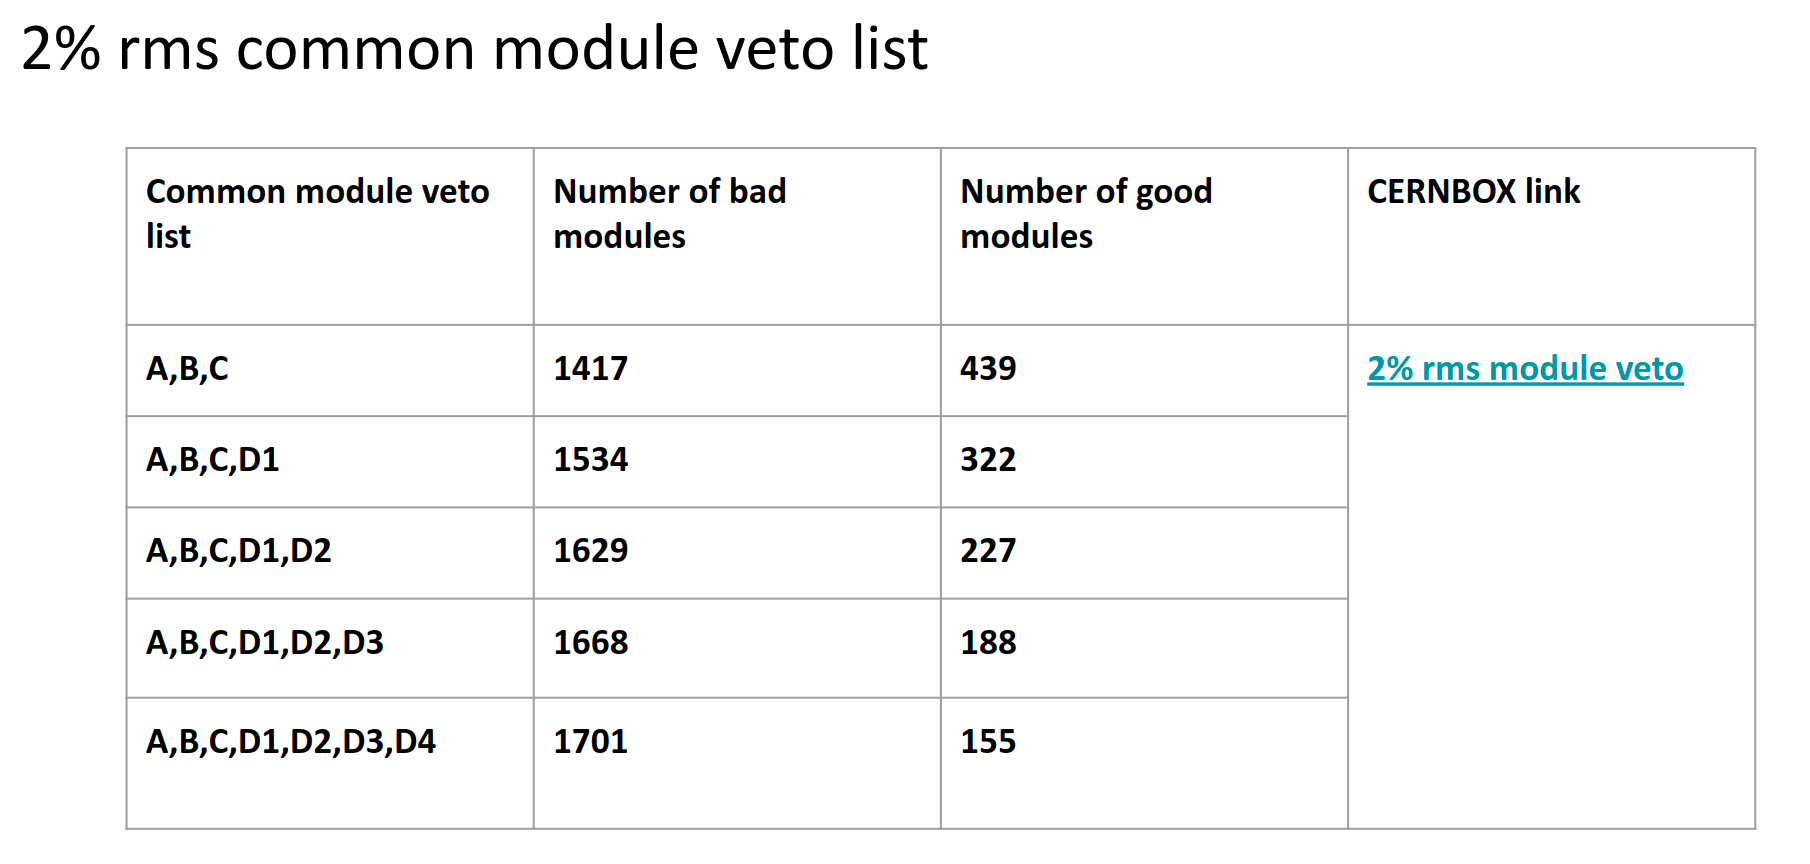
\includegraphics[width=1\textwidth]{ashish_thesis/2per_rms_common_veto.png}
\caption{%
   A method to make 2\% rms common veto.
}
\label{fig:2per common veto}
\end{figure}

\begin{figure}[!htp]
\centering
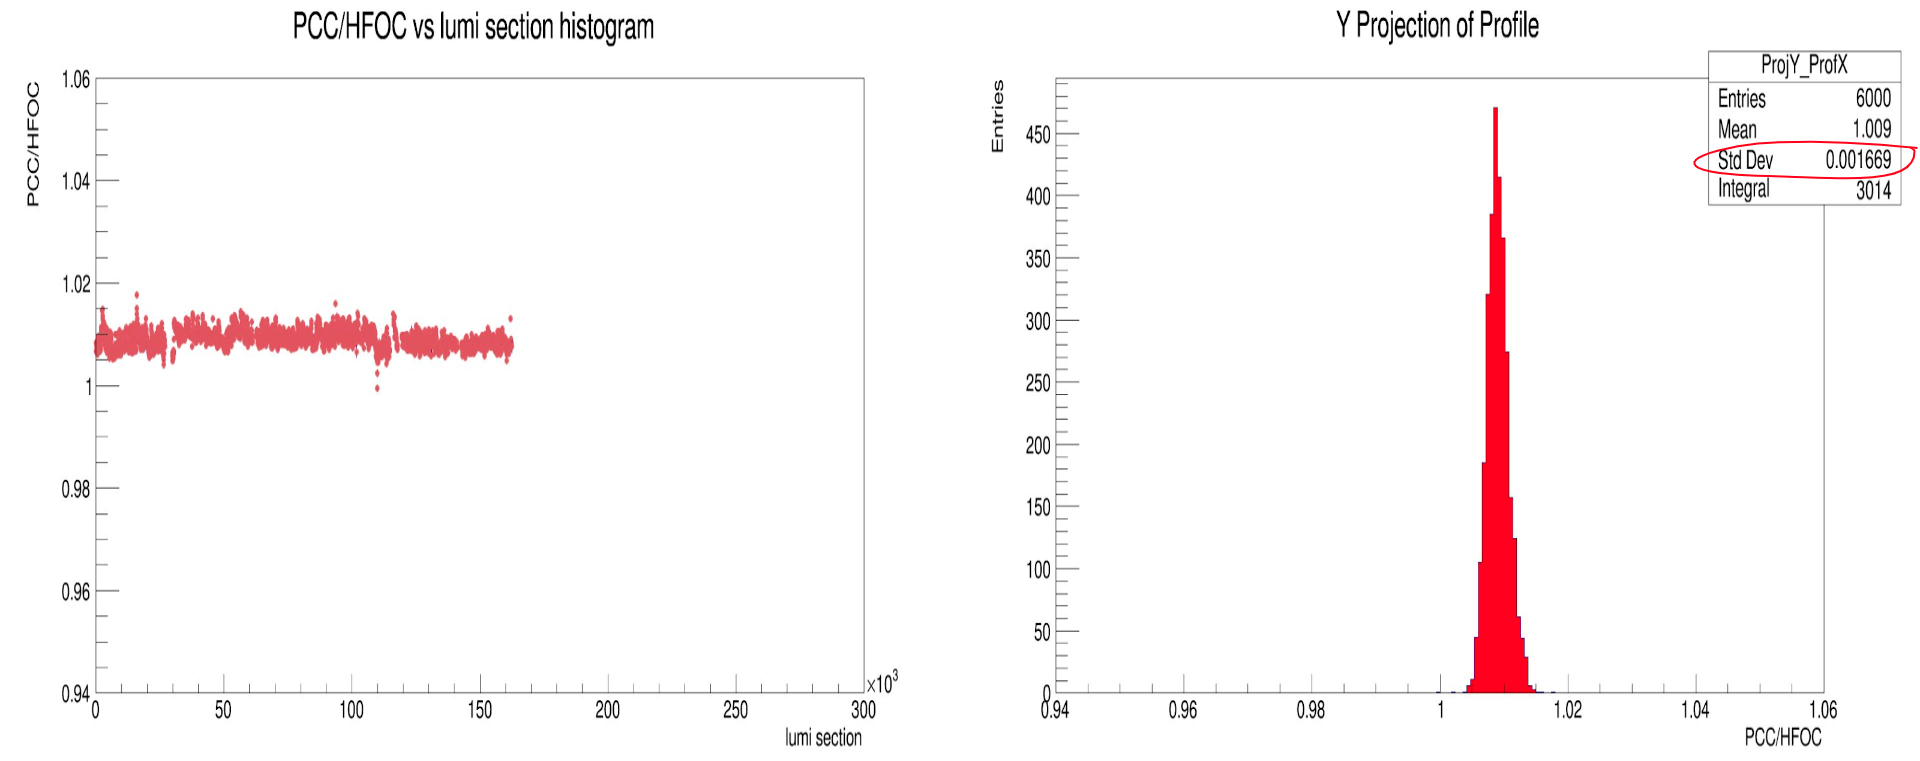
\includegraphics[width=1\textwidth]{ashish_thesis/pcc_hfoc_ratio_stability_2per_common_veto.png}
\caption{%
   Left: X profile of PCC/HFOC luminosity ratio as a function of lumi section for 2\% rms commpon module veto showing instabilities.  Right: Y projection of the X profile of the luminosity ratio. The standard deviation of this projection is taken as the systematic uncertainty due to stability.
}
\label{fig:2per common veto pcc hfoc}
\end{figure}

    
\begin{figure}[!htp]
\centering
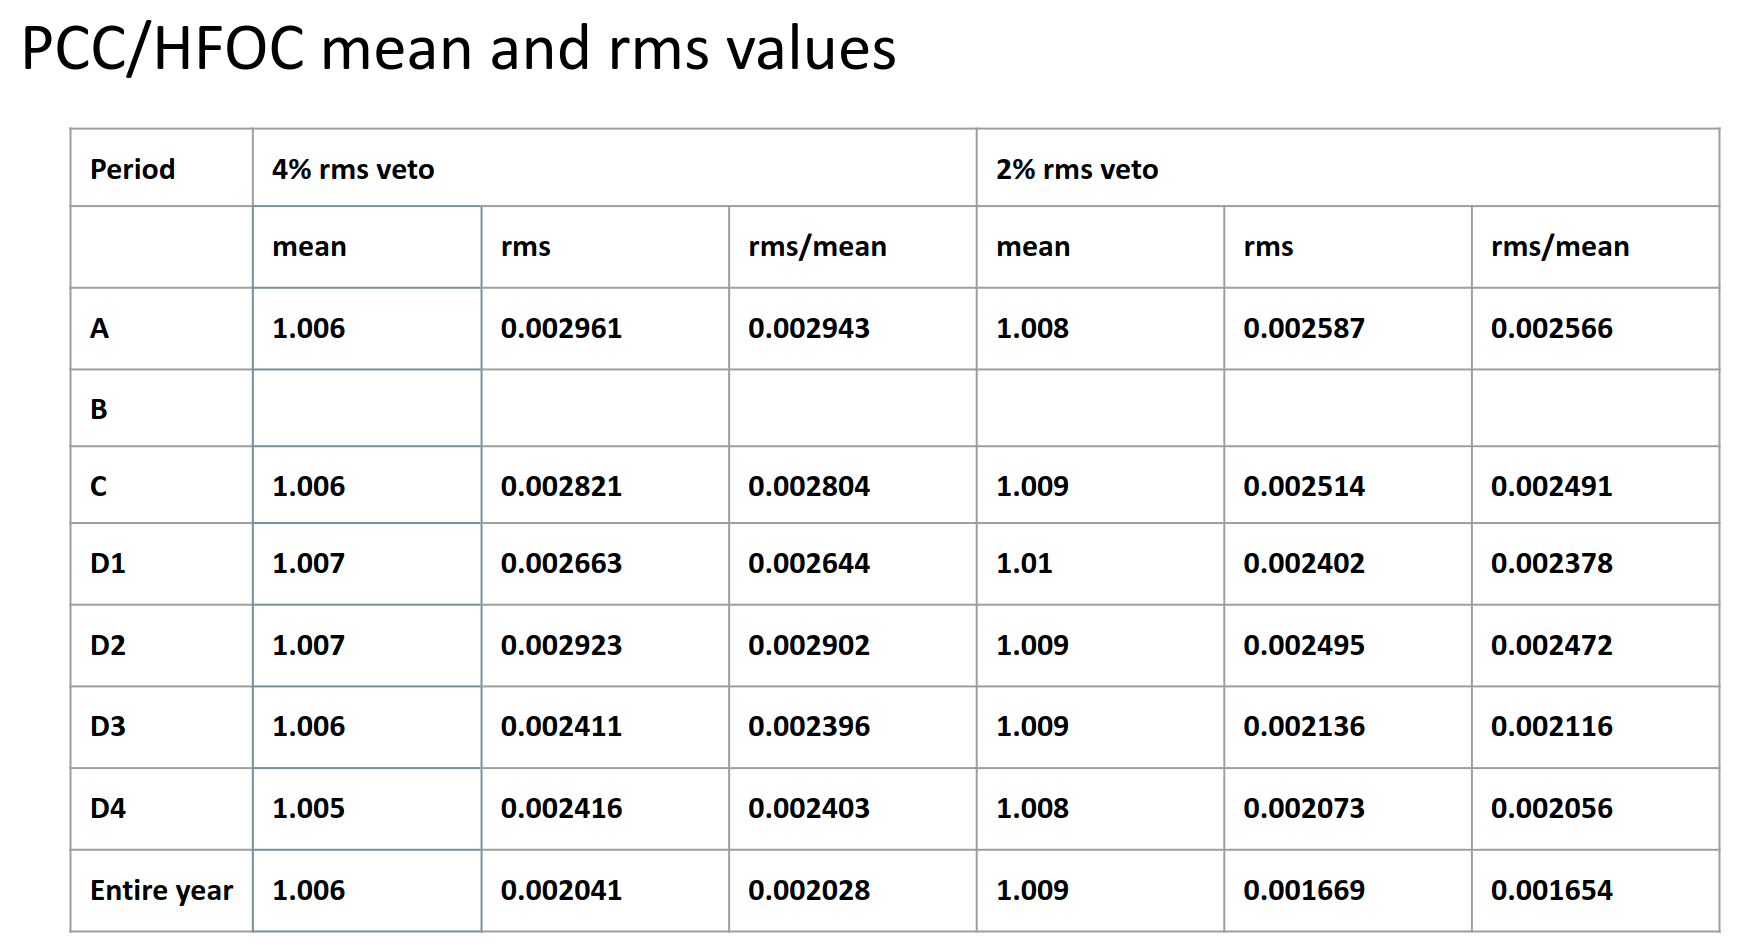
\includegraphics[width=1\textwidth]{ashish_thesis/pcc_hfoc_4_2_rms_mean.png}
\caption{%
  iygjh
}
\label{fig:twoper common veto pcc hfoc rms mean}
\end{figure}

\begin{table}[!ht]
\centering
\topcaption{%
    A method to make 4\% rms commpon module vetolist.
}
\begin{tabular}{ccccc}
    \textbf{Period} & \textbf{# bad modules} & \textbf{# good modules} \\ \hline
    A & 1293 & 563  \\
    B & 1421  & 435  \\
    C & 1522  & 334 \\
    D1 & 1574  & 282  \\
   D2  & 1615  & 241 \\
\end{tabular}
\label{tab:pccvis_diffveto}
\end{table}



\begin{figure}[!htp]
\centering
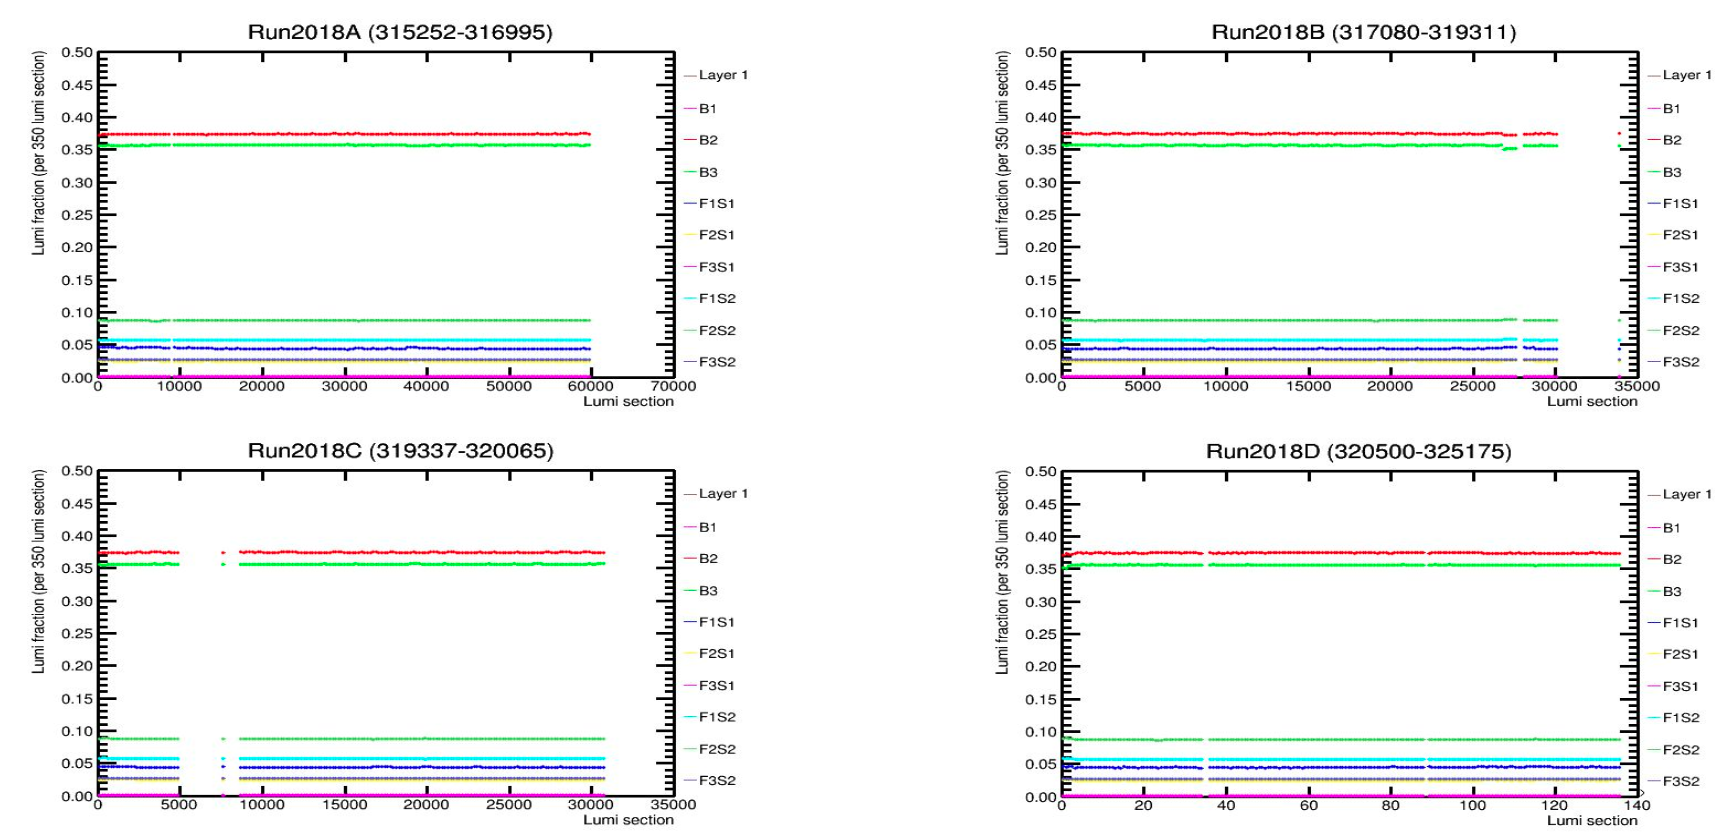
\includegraphics[width=1\textwidth]{ashish_thesis/pcc_layer_disk_stability_2per_veto.png}
\caption{%
PCC stability plots for each layer/Disk for all period using 2\% rms common module veto.
}
\label{fig:pcclayerdisktwopercommonveto}
\end{figure}

\begin{figure}[!htp]
\centering
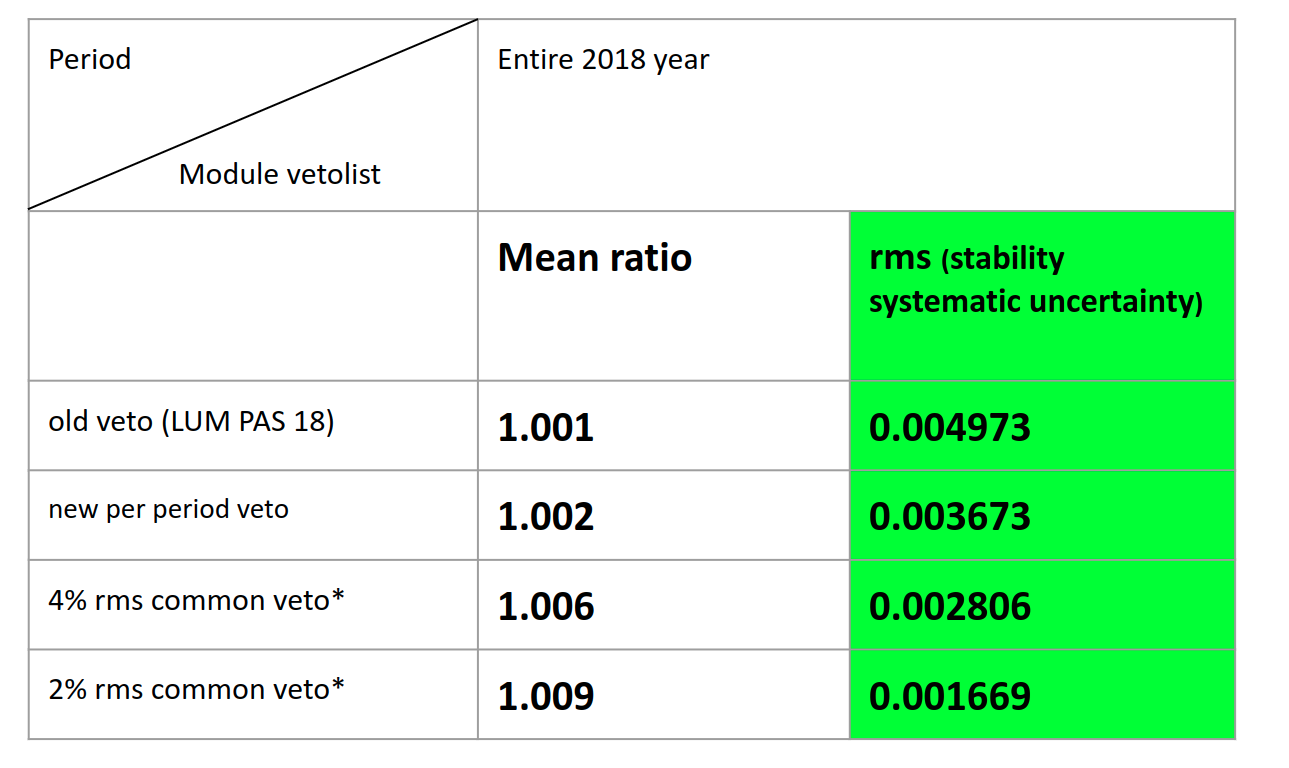
\includegraphics[width=1\textwidth]{ashish_thesis/stability_unc_diff_veto.png}
\caption{%
stability uncertainty all vetoes
}
\label{fig:stabilityuncallveto}
\end{figure}


\begin{figure}[!htp]
\centering
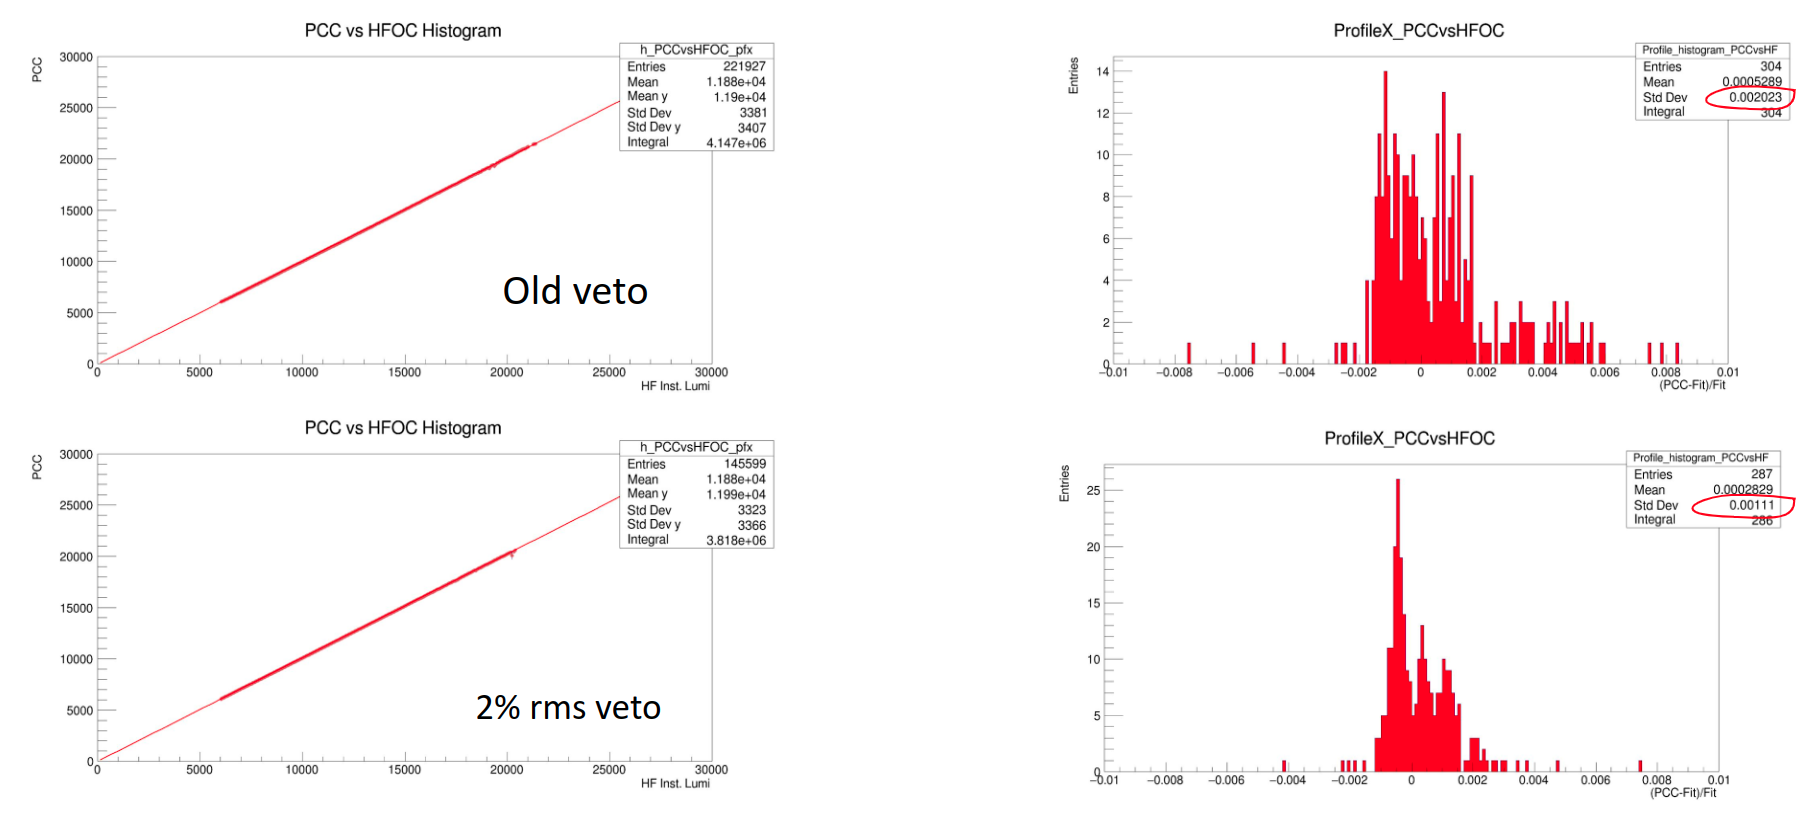
\includegraphics[width=1\textwidth]{ashish_thesis/pcc_hfoc_linearity_sys_unc.png}
\caption{%
linearity systematic uncertainty
}
\label{fig:linearitypcchfoc}
\end{figure}

\begin{figure}[!htp]
\centering
\includegraphics[width=1\textwidth]{ashish_thesis/pcc_hfoc_new_veto_linearity.png}
\caption{%
old new veto linearity
}
\label{fig:pcc_hf_new_lin}
\end{figure}

\begin{figure}[!htp]
\centering
\includegraphics[width=1\textwidth]{ashish_thesis/pcc_hfoc_linearity_sys_unc_2per_common_veto.png}
\caption{%
linearity 2 percent veto
}
\label{fig:linearity2perveto}
\end{figure}


\begin{figure}[!htp]
\centering
\includegraphics[width=1\textwidth]{ashish_thesis/lineairty_diff_veto_sys_unc.png}
\caption{%
all veto linearity sys uncertainty
}
\label{fig:linearitysys}
\end{figure}

\begin{figure}[!htp]
\centering
\includegraphics[width=1\textwidth]{ashish_thesis/pcc_layer_disk_stability_4_commonveto.png}
\caption{%
4 percent veto
}
\label{fig:4perdisklayerstab}
\end{figure}

\begin{figure}[!htp]
\centering
\includegraphics[width=1\textwidth]{ashish_thesis/pcc_layer_disk_mean_rms.png}
\caption{%
pcc layer disk mean rms
}
\label{fig:pixellalyerdiskmeanrms}
\end{figure}


\begin{figure}[!htp]
\centering
\includegraphics[width=1\textwidth]{ashish_thesis/lineairty_diff_veto_period_variation_slope.png}
\caption{%
linearity all period
}
\label{fig:linearityperperiod}
\end{figure}


\begin{figure}[!htp]
\centering
\includegraphics[width=1\textwidth]{ashish_thesis/type1_type2_af_residuals_oldveto_oldp.png}
\caption{%
residuals af
}
\label{fig:afres}
\end{figure}


%\end{comment}
